\documentclass[BTech]{iitmdiss}
\usepackage{textcomp}
\usepackage{times}
\renewcommand{\ttdefault}{cmtt}  % use Computer Modern teletype instead of Courier
\usepackage{tabularx}
\usepackage{url}
\usepackage{rotating}
%\usepackage{adjustbox}
\usepackage{mathtools}
%\usepackage{pbox}
%\usepackage{multirow}
\usepackage{float}
\usepackage{t1enc}
%\usepackage{wrapfig}
\usepackage{graphicx}
\usepackage{epstopdf}
\usepackage{booktabs}
\usepackage{amsmath}
\usepackage{amssymb}
\usepackage{amsfonts}
\usepackage{xcolor}
\usepackage[driverfallback=dvipdfm]{hyperref}

\graphicspath{{figures/}{figures/live_demo/}}

\begin{document}

%%% TITLE
\title{Multimodal Sensing of Operator Pairs: A Dual-Eye-Tracking Pipeline for Coordination-Failure Prediction}
\author{Arya Sikder}
\date{May 2026}
\department{Chemical Engineering}
\newgeometry{left=1in,right=1.5in,top=1in,bottom=0.667in}
\maketitle

%%% CERTIFICATE
\certificate
\vspace*{0.5in}
\noindent This is to certify that the thesis titled
{\bf Multimodal Sensing of Operator Pairs: A Dual-Eye-Tracking Pipeline for Coordination-Failure Prediction},
submitted by {\bf Arya Sikder}, to the Indian Institute of Technology Madras for the award of the degree of
{\bf Bachelor of Technology}, is a bona fide record of the research work done by him under my supervision.
The contents of this thesis, in full or in parts, have not been submitted to any other Institute or
University for the award of any degree or diploma.

\vspace*{1.0in}

\begin{singlespacing}
\hspace*{-0.25in}
\parbox{2.5in}{
\noindent {\bf Prof.\ Rajagopalan Srinivasan} \\
\noindent Research Guide \\
\noindent \textit{Professor} \\
\noindent Dept.\ of Chemical Engineering \\
\noindent IIT Madras, 600 036
}
\hspace*{1.5in}
\parbox{2.5in}{
\vspace*{0.3in}
\noindent Place: Chennai \\
Date: May 2026
}
\end{singlespacing}

%%% ACKNOWLEDGEMENTS
\newgeometry{left=1.5in,right=1in,top=1in,bottom=0.667in}
\acknowledgements

I am grateful to my research guide, Prof.\ Rajagopalan Srinivasan, for his guidance and for the freedom to pursue this line of work. I thank the 47 pairs of student participants who contributed their time to the recording sessions, and the lab staff who supported the six-modality recording protocol. The analysis benefited from open-source contributions to scikit-learn, LightGBM, XGBoost, PyRQA and matplotlib.

\vspace*{0.4in}
\noindent\textbf{Code and data availability.} The two code repositories accompanying this thesis are openly released and span the full apparatus-to-analysis pipeline:

\begin{itemize}
\item \textbf{Experiment user interface and data-collection stack} (React/TypeScript Director-Matcher application, Express WebSocket backend, WearOS heart-rate streaming app):\\
\texttt{\href{https://github.com/valiant-disciple/map-task}{https://github.com/valiant-disciple/map-task}}
\item \textbf{Analysis pipeline} (preprocessing, feature engineering, predictor, failure-mode clustering, figure-generation, and the LaTeX source of this thesis):\\
\texttt{\href{https://github.com/valiant-disciple/operator-pair-analysis}{https://github.com/valiant-disciple/operator-pair-analysis}}
\end{itemize}

\noindent The raw participant data are held separately under the study's ethics protocol and are not included in either repository; they are available from the author on reasonable request.

%%% ABSTRACT
\abstract
\noindent KEYWORDS: \hspace*{0.5em} \parbox[t]{4.4in}{operator monitoring; dyadic coordination; multimodal physiological sensing; dual eye-tracking; joint visual attention; cardiac synchrony; failure-mode taxonomy; workload composites.}

\vspace*{24pt}
\noindent
Safety-critical work in chemical process plants is rarely the job of a single operator. The board operator at the console and the field operator on the unit coordinate through a continuous verbal channel over a shared mental model of the plant, and incident reviews across the petrochemical industry are consistent in implicating the link between operators rather than failure of either operator alone. The coordination axis between the two operators, in other words, carries an outsized share of the risk in process safety, and it is the axis that single-operator monitoring instruments cannot see. This thesis is a methodological precursor to operator-pair monitoring for chemical-engineering control rooms. It develops, on a laboratory analogue of the board-field coordination problem (an instructor-and-follower map task in which one operator verbally guides the other along a route under a shared spatial referent), the sensing apparatus, feature pipeline, and predictive model that the chemical-engineering deployment will require. Five operator-side modalities are recorded synchronously from both members of the pair: cardiac, gaze, audio, post-task survey, and per-trial dialogue annotation. Two screen-mounted eye-trackers operate in parallel (one per operator), and both gaze streams are projected into a shared map coordinate frame so that joint visual-attention measures across the role-asymmetric operators become definable. On forty pairs, the multimodal predictor reaches a cross-pair AUC of $0.76$ for trial-level coordination-failure prediction on previously unseen pairs, against $0.65$ for the best single modality. Three within-pair-normalised workload composites characterise per-operator and pair-level cognitive load, and a four-mode physiology-derived failure-mode taxonomy (Director-Overloaded, Matcher-Disengaged, Director-Disengaged, and Calm-Decoupled) decomposes the predictor's failure surface into operator-side mechanisms that map directly onto the overload and vigilance-decrement constructs of the abnormal-situation-management literature. Joint cardiac coupling separates failure from success at Cohen's $d \approx 0.7$ across three independent coupling features, indicating that even the lowest-friction operator-side sensor in a control-room deployment, the wrist smartwatch on both operators, would already carry meaningful coordination-state information. The contribution of this thesis is therefore three-fold: a multimodal sensing apparatus that resolves the role-asymmetric dual eye-tracking problem; an empirical demonstration that operator-pair coordination failure is predictable at trial-level resolution from a heterogeneous reference cohort; and a failure-mode taxonomy and workload-composite framework that maps onto the constructs already used in chemical-engineering process-safety monitoring, against which a confirmatory study with trained plant operators is the natural next step. Apparatus design, feature pipelines, and analysis code are released alongside the thesis to support that confirmatory study and subsequent operational deployment, at \href{https://github.com/valiant-disciple/map-task}{\texttt{github.com/valiant-disciple/map-task}} (experiment UI and data-collection stack) and \href{https://github.com/valiant-disciple/operator-pair-analysis}{\texttt{github.com/valiant-disciple/operator-pair-analysis}} (analysis pipeline and thesis source).


\pagebreak

\disclaimer
The Department of Chemical Engineering, IIT Madras and the staff of IIT Madras do not accept any responsibility for the truth, accuracy or completeness of material contained within or associated with this dissertation.

Persons using all or any part of this material do so at their own risk, and not at the risk of the Department of Chemical Engineering, IIT Madras and the staff of IIT Madras.

This document, the associated hardware, software, drawings, and other material set out in the associated appendices should not be used for any other purpose: if they are so used, it is entirely at the risk of the user.

\pagebreak

%%% TOC, LoT, LoF
\begin{singlespace}
\tableofcontents
\thispagestyle{empty}
\listoftables
\addcontentsline{toc}{chapter}{LIST OF TABLES}
\listoffigures
\addcontentsline{toc}{chapter}{LIST OF FIGURES}
\end{singlespace}

%%% ABBREVIATIONS
\newpage
\begin{tabbing}
\end{tabbing}
\abbreviations
\noindent
\begin{tabbing}
xxxxxxxxxxxxxx \= xxxxxxxxxxxxxxxxxxxxxxxxxxxxxxxxxxxxxxxxxxxxxxxx \kill
\textbf{AUC} \> Area Under the (ROC) Curve \\
\textbf{AOI} \> Area Of Interest \\
\textbf{BPM} \> Beats Per Minute \\
\textbf{CRQA} \> Cross-Recurrence Quantification Analysis \\
\textbf{CV}  \> Cross-Validation \\
\textbf{GroupKFold} \> Group-aware K-fold cross-validation \\
\textbf{HR}  \> Heart Rate \\
\textbf{HRV} \> Heart Rate Variability \\
\textbf{ICC} \> Intraclass Correlation Coefficient \\
\textbf{LLM} \> Large Language Model \\
\textbf{MdRQA} \> Multidimensional Recurrence Quantification Analysis \\
\textbf{NASA-TLX} \> NASA Task Load Index \\
\textbf{PCA} \> Principal Component Analysis \\
\textbf{PSMM} \> Perceived Shared Mental Model \\
\textbf{RMSSD} \> Root Mean Square of Successive Differences \\
\textbf{SHAP} \> SHapley Additive exPlanations \\
\textbf{W$_D$, W$_M$, W$_{\text{team}}$} \> Director / Matcher / pair-level workload composites \\
\end{tabbing}

\pagebreak

%%% NOTATIONS
\chapter*{\centerline{NOTATIONS}}
\addcontentsline{toc}{chapter}{NOTATIONS}
\begin{singlespace}
\begin{tabbing}
xxxxxxxxxxxx \= xxxxxxxxxxxxxxxxxxxxxxxxxxxxxxxxxxxxxxxxxxxx \kill
$n$         \>  Number of trials \\
$n_+$       \>  Number of failure trials (positive class) \\
$d$         \>  Cohen's $d$ effect size \\
$\rho$      \>  Spearman rank correlation \\
$\alpha_1$  \>  Detrended-fluctuation-analysis short-term scaling exponent \\
$k$         \>  Number of K-means clusters \\
$B$         \>  Bootstrap resample count \\
\end{tabbing}
\end{singlespace}

\pagebreak
\clearpage
\pagenumbering{arabic}

%%% MAIN BODY (Introduction, Methods, Results, Discussion, Conclusion)
\chapter{INTRODUCTION}
Safety-critical work in chemical process plants is rarely the job of a single operator. The board operator at the distributed-control-system console sees the full plant graphic, the alarm queue, and the setpoint trends; the field operator on the unit sees the actual equipment, valves, and local indicators. The two coordinate by radio over a shared mental model of the plant, and during abnormal situations (startups, shutdowns, alarm floods, and unit upsets) it is the field-board pair, rather than either operator alone, that determines whether the disturbance is contained or escalates \cite{bullemer1996abnormal,nimmo1998abnormal,nazir2012role}. Incident reviews across the petrochemical and refining industries are consistent in implicating the link between operators rather than failure of either operator individually. Human factors are implicated in over two-thirds of major industrial accidents \cite{reason1990human,kletz2001learned}; how those factors play out in the joint state, rather than inside either operator, is what this thesis is built to measure. The same role-asymmetric pair structure shows up in aviation (captain and first officer under crew resource management protocols \cite{helmreich1999evolution,kanki2010crew}) and in surgery (lead surgeon and scrub nurse \cite{undre2007teamwork,catchpole2008teamwork}), but the chemical-engineering control room is the domain to which the methodology developed in this thesis is directly addressed.

The trouble is that the standard operator-monitoring toolkit, including the toolkit used in chemical-engineering process-safety research, was built around a single observer \cite{wickens2008model,parasuraman2008situation}. Gaze entropy and fixation dispersion separate experts from novices on chemical-plant simulators \cite{bhavsar2017eye,sharma2016eye,shahab2021metrics}. Adding EEG to single-operator eye-tracking improves cognitive-workload classification in training environments \cite{iqbal2024multi,iqbal2020dynamic}. Pupillometry, dwell time, the NASA Task Load Index \cite{hart1988development} and Endsley's situation-awareness framework \cite{endsley1995toward} round out what most field deployments lean on. None of it watches both operators at once. So the construct that matters most for chemical-engineering field deployment, the state of the board-field pair, is the one that current sensing does not actually see. This thesis is a methodological precursor to closing that gap.

Three largely disjoint literatures bear on the joint state. The first is cardiac synchrony. Verdi\`ere \emph{et al.}~\cite{verdiere2020thms} introduced a delayed-coincidence-count measure of inter-operator heart-rate coupling on a cooperative microworld task in this journal. Sharika \emph{et al.}~\cite{sharika2024heart} reported, more recently, that interpersonal heart-rate synchrony from multidimensional recurrence quantification of group heart-rate signals predicts the probability of 44 hidden-profile groups reaching the correct consensus decision at over 70\% cross-validation accuracy. That is, as far as we know, the closest predictive precedent in the literature. The second thread is dual eye-tracking. Richardson and Dale \cite{richardson2005looking} established speaker--listener gaze coupling. Schneider, Brennan and colleagues \cite{schneider2018leveraging,brennan2008coordinating,ho2021gaze} have used joint visual attention to predict collaborative-learning quality. The third thread is hyperscanning with functional near-infrared spectroscopy, where inter-brain coherence is observed to rise during cooperative tasks \cite{cui2012nirs,dumas2010interbrain,czeszumski2020hyperscanning}. Each thread looks at the joint state through one sensor family. Recent multimodal team-physiology work \cite{li2025physiological} combines cardiac and respiration signals across operators. Trial-level prediction of coordination failure under a dyad-disjoint protocol, which is the protocol any chemical-engineering control-room deployment would actually face, has not, to our reading, been an explicit target of these earlier studies.

The work reported in this thesis is therefore positioned as the laboratory precursor to a chemical-engineering operator-pair monitoring system. The laboratory analogue chosen is the HCRC Map Task \cite{anderson1991hcrc,carletta1996hcrc}, which preserves the structural features that make the chemical-engineering board-field pair hard to monitor: role asymmetry (instructor and follower), a shared spatial referent (the map, analogous to the plant graphic), a continuous verbal channel (analogous to the radio link), and an outcome that depends on the link between operators rather than on either operator alone. The script is the same on every trial. One operator (the Director, mapping onto the board operator) sees a full street-style map with the target route highlighted, and gives verbal directions. The other operator (the Matcher, mapping onto the field operator) sees only the map outline on a blank canvas, and draws the route in response. The trial fails if the Matcher's drawn path does not reach the target. Five operator-side modalities are recorded in synchrony per trial: the cardiac signal from a wrist-worn smartwatch, from which frequency-domain heart-rate variability indices are derived; dual screen-mounted eye-tracking (Aurora ET for the Director at $\sim$$120$~Hz, SmartEye Pro 10 for the Matcher at $60$~Hz); per-operator audio, with word-level Whisper alignment \cite{radford2023whisper}; post-task survey responses; and per-trial dialogue annotations produced by a reasoning language model \cite{openai2025gpt5}. Each of these modalities has a chemical-engineering control-room analogue: the smartwatch is the lowest-friction wearable; the dual-tracker setup transposes to two screens watching the same plant graphic; and the audio plus dialogue-annotation stack transposes to the radio channel between operators. Under dyad-disjoint cross-validation, the multimodal predictor reaches AUC of $0.761$ against a best single-modality AUC of $0.654$ on the laboratory analogue.

The dual eye-tracking configuration is the apparatus piece on which the chemical-engineering deployment hinges. Two screen-mounted trackers operate in parallel (one per operator), and both gaze streams are projected into a common map coordinate frame. The role asymmetry of the task, which mirrors the asymmetry between the board and field operators in a control room, rules out the standard single-tracker setup. In a control-room deployment the corresponding shared frame would be the plant graphic on the DCS console (which the field operator can also pull up on a tablet), and the joint-gaze features would index the extent to which the two operators are looking at the same unit, alarm, or trend at the same time. This is, in the language of the operator-monitoring literature, an instrumented version of shared situation awareness \cite{endsley1995toward,salmon2008what,stanton2017state}.

Three within-pair-normalised workload composites characterise per-operator and pair-level cognitive load, and a four-mode physiology-derived failure-mode taxonomy decomposes the predictor's failure surface into operator-side mechanisms (Director-Overloaded, Matcher-Disengaged, Director-Disengaged, Calm-Decoupled) that map onto overload and vigilance-decrement constructs already in use in the chemical-engineering process-safety literature \cite{bhavsar2017eye,iqbal2024multi,iqbal2020dynamic}. The contribution of this thesis is therefore three-fold. First, the dual eye-tracking apparatus makes joint visual-attention measures across role-asymmetric operators definable in a task family in which they have not previously been defined. Second, the broader multimodal sensing pipeline (cardiac, gaze, audio, survey, and per-trial LLM dialogue annotation) recovers a trial-level coordination-failure AUC of $0.76$ on previously unseen pairs under dyad-disjoint cross-validation, against $0.65$ for the best single modality. Third, the failure-mode taxonomy and workload-composite framework decompose that prediction into operator-side mechanisms that map directly onto the constructs already used in chemical-engineering process-safety monitoring, against which a confirmatory study with trained plant operators is the natural next step (Chapter~\ref{sec:future}). Apparatus design, feature pipelines, and analysis code are released alongside the thesis to support that confirmatory study and subsequent operational deployment.

Section~\ref{sec:methods} describes the apparatus, task, and evaluation protocol. Section~\ref{sec:results} reports the four contributions in turn (Sections~\ref{sec:multimodal} through \ref{sec:modes}), followed by supporting analyses in Section~\ref{sec:supporting}. Section~\ref{sec:discussion} discusses deployment implications and limitations, with Section~\ref{sec:cheme} mapping the laboratory results onto the chemical-engineering control room. Chapter~\ref{sec:future} sets out the validation, sensor-reduction, and scope-expansion directions needed to take the present work to operational deployment.


\chapter{METHODS}\label{sec:methods}

\section{Participants and Task}
We recruited 47 pairs of student participants. Seven pairs were excluded owing to sensor failure or incomplete data, yielding 40 clean pairs and 225 data trials for analysis. Two additional pairs were excluded from analyses requiring full coverage across all six modalities, and these exclusions are flagged in the dataset metadata. Sample size was determined by the logistical demands of the six-modality recording protocol rather than by an a priori power calculation. It nonetheless falls within the range of the closest predictive precedents in the literature, 50 pairs in Verdi\`ere \emph{et al.}~\cite{verdiere2020thms} and 44 groups in Sharika \emph{et al.}~\cite{sharika2024heart}.

Each pair completed 8 trials of 210~s, of which the first two served as warm-up and the remaining six contributed to the analysed dataset. The task, which we refer to throughout as the Director--Matcher paradigm, is an instructor-and-follower map task adapted from the HCRC Map Task corpus \cite{anderson1991hcrc,carletta1996hcrc,brown1984teaching}. The two operators see the same underlying map under deliberately asymmetric presentations (Figure~\ref{fig:maps}). The Director was shown a full street-style map with the target route highlighted in red, whereas the Matcher viewed only the same map's landmark outline (no route) rendered on a $651 \times 900$ pixel blank canvas. The Director gave verbal instructions on a live audio channel; the Matcher drew the corresponding path on the canvas. Path completion was scored against the highlighted route on the Director's view; the Matcher never saw the highlighted route during the trial. The role asymmetry of the task is deliberate, and mirrors the asymmetry between the board operator (full plant graphic on the DCS console) and the field operator (local indicators on the unit) in a chemical-engineering control room.

\begin{figure}[!t]
\centering
\begin{minipage}[t]{0.46\textwidth}
\centering
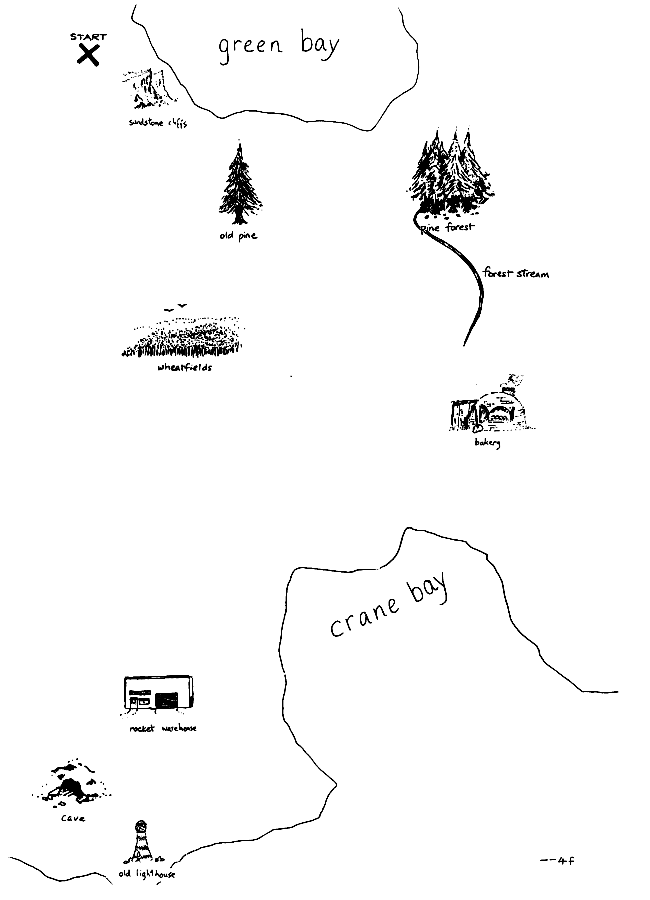
\includegraphics[width=\textwidth]{map_director_example.png}
\\[2pt]
{\small (a) Director view (full map with target route highlighted)}
\end{minipage}\hfill
\begin{minipage}[t]{0.46\textwidth}
\centering
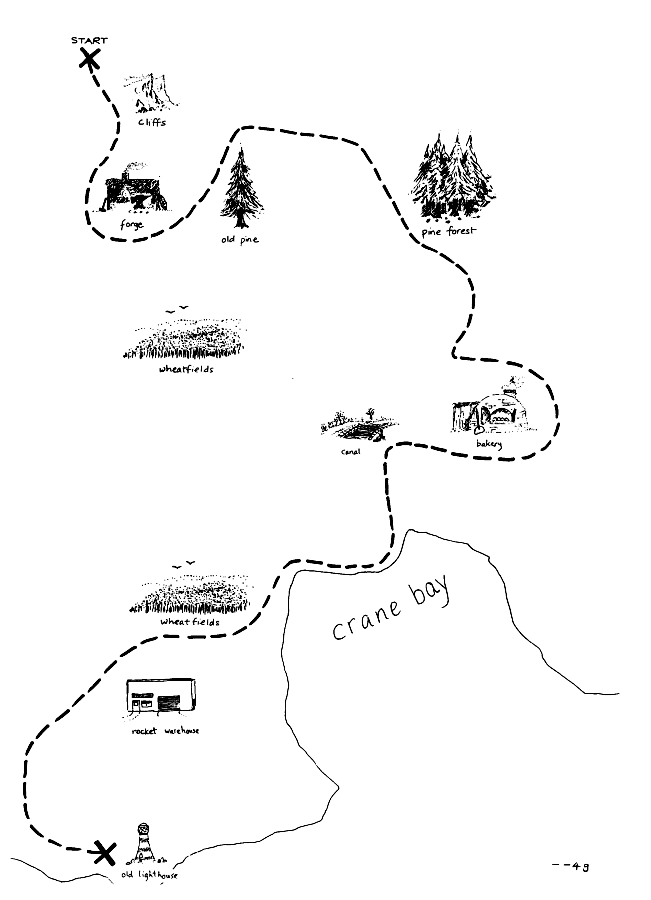
\includegraphics[width=\textwidth]{map_matcher_example.png}
\\[2pt]
{\small (b) Matcher view (landmark outline only, blank canvas)}
\end{minipage}
\caption[Director and Matcher map views]{Director and Matcher map views, example trial. The Director (instructing operator) sees the full map with the target route highlighted in red and gives verbal directions over a live channel. The Matcher (following operator) sees only the landmark outline on a blank canvas and draws the route in response. The role asymmetry mirrors the asymmetry between the board operator (full plant graphic) and the field operator (local indicators only) in a chemical-engineering control room.}
\label{fig:maps}
\end{figure}

Two protocol constraints structure the coordination problem: the Director's view never included the Matcher's evolving drawing, and spatially grounded pointing or other deictic reference was precluded, so that speech remained the sole channel of coordination. Trial outcome was operationalised as a binary variable, \texttt{target\_reached} $=$ \texttt{false}, assigned when the Matcher's drawn path did not reach the Director's target node by the end of the trial. We refer to this outcome as coordination failure. The label captures the construct through the task's primary behavioural outcome alone; richer constructs such as shared-mental-model breakdown \cite{cannonbowers1993shared,mohammed2010metaphor} or joint situation-awareness loss \cite{salmon2008what,stanton2017state} were not directly measured.

\section{Apparatus}
Each pair was recorded synchronously across six operator-side modalities (Table~\ref{tab:modalities}). The cardiac signal was acquired from a wrist-worn smartwatch on each operator, broadcasting beat-per-minute samples at an irregular rate near $0.5$~Hz (median inter-sample interval $\approx 2$~s, mixed $1$-s and $2$-s broadcasts). The standard per-trial frequency-domain HRV indices (RMSSD, LF and HF power, sample entropy, and detrended-fluctuation-analysis $\alpha_1$) were computed after interpolating the inter-beat-interval series to a uniform $4$~Hz grid \cite{shaffer2017hrv,shaffer2014healthy,task1996heart}. Per-operator audio was captured at 16~kHz on lapel microphones and aligned at the word level with Whisper \cite{radford2023whisper}. From these aligned transcripts, lexical, prosodic and event-level descriptors were derived, covering disfluency, repair and reference structure; repair events, in particular, were classified along the conversation-analytic taxonomy of \cite{schegloff1977preference,schegloff1992repair}. The NASA Task Load Index \cite{hart1988development,hart2006nasa} and a perceived-shared-mental-model survey \cite{cooke2003measuring,mathieu2000influence} were administered after every trial. Finally, each per-trial transcript was passed to gpt-5-mini \cite{openai2025gpt5} at maximum reasoning effort with a structured-output prompt returning per-trial JSON for the route plan, repair sequences, common-ground events, misalignment events, errors, dropouts and a free-form failure-mode description (Section~\ref{sec:llm-anno}). The Matcher's stroke-level drawing was retained for outcome scoring only, and was not fed into any predictive analysis.

\begin{table}[!t]
\caption[Operator-side recording stack]{Operator-side recording stack. Five modalities feed the predictor; the sixth (stroke-level drawing) is captured for outcome scoring only.}
\label{tab:modalities}
\centering
\small
\begin{tabular}{lll}
\toprule
Modality & Device / source & Native rate \\
\midrule
Cardiac & Wrist-worn smartwatch (both operators) & $\sim$$0.5$~Hz (irregular) \\
Director gaze & Aurora ET (iMotions, screen-mounted) & $\sim$$120$~Hz \\
Matcher gaze & SmartEye Pro 10 (screen-mounted) & $60$~Hz \\
Per-operator audio & Lapel microphone, Whisper alignment & 16~kHz \\
Self-report & NASA-TLX + perceived-SMM survey & Per trial \\
Dialogue annotation & gpt-5-mini structured JSON & Per trial \\
\midrule
Drawing (excluded) & Stroke-level capture for scoring & Per stroke \\
\bottomrule
\end{tabular}
\end{table}

Of particular interest is the dual eye-tracking configuration, which constitutes the novel piece of the apparatus and is dictated by the role asymmetry inherent to the task. Both eye-trackers were screen-mounted (fixed) and configured per operator: the Director was tracked with an Aurora ET unit (iMotions stack) at a native rate near $120$~Hz, and the Matcher with a SmartEye Pro 10 unit at $60$~Hz \cite{holmqvist2011eye,holmqvist2023eye,niehorster2024reporting}. Taken in isolation, each tracker appears to be the obvious choice for its operator. The two together, however, yield gaze in two unrelated reference frames. In order to render the streams comparable, both raw gaze trajectories were mapped to a common $651 \times 900$ map-space coordinate system through a per-participant nine-point calibration performed at the start of each session. The joint-gaze feature family employed in the analyses below follows directly from such an alignment, and comprises cross-recurrence quantification on the joint trajectory, joint area-of-interest fixation, gaze convergence within a fixed radius, and gaze leader/follower lag derived from the cross-recurrence diagonal. None of these features could be defined on a single-tracker setup. Nor, indeed, could they be defined on two trackers in the absence of a shared frame.

A single wall-clock anchor was recorded at trial onset and used offline to align the modalities, which run on independent clocks (two trackers, separate audio, and a smartwatch HR broadcast). Per-operator features were computed on each modality's native rate; pair-level features were then computed on common analysis grids that depend on the family (joint cardiac coupling on a $1$~Hz grid; joint gaze coupling on a $10$~Hz grid; cross-modal pupil--HR coupling on a $1$~Hz grid). The residual drift across a 210-s trial remains small relative to the 30-s analysis window, and is in any case absorbed by the recurrence-based joint features, which are insensitive to small constant offsets along the cross-recurrence diagonal.

\section{Language-Model Dialogue Annotation}\label{sec:llm-anno}
Unlike the other modalities, the dialogue annotation produces a structured natural-language object per trial rather than a continuous time series, so we describe it separately. We passed each per-trial transcript (already word-aligned by Whisper) to gpt-5-mini \cite{openai2025gpt5} at maximum reasoning effort, prompting it for a structured JSON output. We asked the model to fill in eight fields. One field carries an inferred route plan that we reconstruct from the Director's instructions. A second carries the sequence of repair events, tagged with type and initiator. A third tracks common-ground updates, listing which landmarks became mutually known and at what point in the trial they did so. A fourth tracks misalignment events: places in the dialogue where the Director and the Matcher appeared to refer to different objects. Two further fields carry model-flagged errors and dropouts, which we treat as candidates rather than as ground truth, together with a one- to two-sentence free-form failure-mode description. In practice, we use the structured count-style fields directly as per-trial predictor features (repair counts, misalignment counts, and so on). The free-form description, by contrast, is reserved for the content-mode clustering reported in Section~\ref{sec:modes}. Of note, we have not benchmarked the LLM-derived annotation against blinded human coders here, and we do not claim it as a substitute for trained human coding; what we do claim is a descriptive enrichment of the dialogue stream beyond what surface acoustic features can recover.

\section{Feature Engineering}
In the present work, two families of features were constructed. Approximately one hundred per-operator features were computed independently on each operator from the cardiac, gaze, audio and survey streams, and their interpretation has been grounded in the standard operator-monitoring scaffolding: prolonged fixation durations have been demonstrated to reflect deeper cognitive processing or elevated task difficulty \cite{henderson2003human,rayner2009eye}; an enlargement of the pupil diameter is taken as an index of cognitive effort \cite{kahneman1973attention,bhavsar2016pupillometry}; and elevated gaze-transition entropy has been associated with exploratory or unsystematic scanning behaviour \cite{bhavsar2017eye,sharma2016eye}. The joint-coupling family was further decomposed into four sub-types. The largest of these, the joint-cardiac coupling, was computed as multidimensional recurrence and cross-recurrence on the bivariate $\langle\text{HR}_D, \text{HR}_M\rangle$ state space \cite{wallot2016beyond,wallot2018tutorial,marwan2007recurrence}. The joint-gaze coupling, rendered tractable only by the deployment of two synchronised eye-trackers in the apparatus, comprises cross-recurrence quantification, the joint area-of-interest fixation rate, gaze convergence within a fixed radius, and a four-dimensional MdRQA computed on the joint $\langle x_D, y_D, x_M, y_M\rangle$ map-space gaze trajectory. Cross-modal coupling was constructed by augmenting the Director gaze with the Matcher heart rate, coupling the Director speech to the Matcher gaze, and applying dynamic time warping over the multivariate joint state. The smallest sub-type, namely the classical phase-locking value, was computed on per-operator pupil and heart-rate signals. Features that are functionals of the outcome were excluded on endogeneity grounds \cite{kapoor2023leakage}; the excluded set comprises the drawing-extent variables, the drawing-kinematic totals, and the post-task spatial-accuracy summaries (Chamfer distance, Hausdorff distance, intersection-over-union, route coverage and landmark coverage). Following this exclusion, the pool fed into the proposed predictor contains 823 non-endogenous features.

Three within-pair-normalised workload composites were subsequently constructed on top of this feature pool, namely a Director composite $W_{\text{director}}$, a Matcher composite $W_{\text{matcher}}$ and a pair-level composite $W_{\text{team}}$. For each composite, the approximately seven hundred raw features in the pool were within-pair z-scored, sign-aligned to the failure outcome on the training partition, and reduced by exploratory analysis to a single summary score per operator together with one summary score for the pair. Within-pair z-scoring has been preferred over raw signals in the present analysis because, over the 30-minute session, the resting heart-rate baselines were observed to be essentially trait-level stable (ICC $= 0.99$), a value that lies within the range reported in the HRV literature for short laboratory sessions \cite{shaffer2017hrv,shaffer2014healthy,laborde2017hrv}. Furthermore, given that the between-pair variance was found to be substantially larger than the within-pair within-session variance, a predictor trained on raw signals would inevitably lock onto pair identity rather than onto the state change of interest. Notably, the proposed normalisation scheme circumvents this confound by construction.

To evaluate model performance, we adopted a 10-fold GroupKFold cross-validation scheme grouped on the dyad, and we repeated the procedure across 3 seeds in order to quantify run-to-run stability. For each seed we report the pooled-fold area under the ROC curve, and across seeds we report the mean $\pm$ standard deviation. To select hyperparameters without leakage, we ran Optuna with twenty trials per outer fold against an inner three-fold dyad-disjoint validation split. Within each training fold, we further applied an mRMR-style feature selection step that retained the top forty features by F-test and subsequently pruned correlated predictors at $|r| < 0.85$ \cite{peng2005feature,ding2005minimum}. We confined standardisation, feature selection, and hyperparameter tuning to the training fold, so that the test dyads' labels never informed any modelling choice. As a robustness check, we additionally ran a 5-fold GroupKFold $\times$ 5 seeds configuration, which converged on the same conclusion.

In order to assess whether the multimodal signal exceeded chance, we further checked it against a within-fold label-shuffle permutation null with 200 within-pair refits \cite{maris2007nonparametric,nichols2002nonparametric}. Furthermore, to quantify the uncertainty of the AUC estimates, we constructed bootstrap confidence intervals using $B = 200$ to 1000 dyad-clustered resamples \cite{efron1987better}.

The headline prediction target was coordination failure, with $n_+ = 73$ failures across 225 trials. In addition, we tabulated eight exploratory secondary targets alongside the primary outcome: four physiology-derived modes obtained from K-means clustering on the principal components of within-pair-z-scored physiology, three top-quartile event-count flags derived from the language-model dialogue annotations, and one language-model content target capturing lexical-mismatch cluster membership.

\section{Statistical Analyses for Secondary Findings}
The modality ablation runs as a separate 5-fold GroupKFold $\times$ 3 seeds pipeline with an F-test top-40 in-fold screen, comparing Director-only, Matcher-only, joint-only and combined feature partitions. The per-task-difficulty stratification uses trial-level difficulty labels derived post-hoc from the map's branching complexity and the route length. The stratification was not pre-registered, and we treat it as a descriptive cut. The workload composites were built by exploratory analysis on the same set on which they are evaluated, and their AUCs are reported in-sample throughout.


\chapter{RESULTS}\label{sec:results}

\section{Multimodal Predictor}\label{sec:multimodal}
We found that a tuned soft-voting ensemble of three gradient-boosting learners reached pooled AUC of $0.761 \pm 0.010$ on coordination failure under 10-fold dyad-disjoint GroupKFold cross-validation across three random seeds (Table~\ref{tab:headline}, Fig.~\ref{fig:multimodal}). Speech was the best single modality, at AUC $0.654$. Cardiac features alone fell below chance, at AUC $0.457$. The reason for that last number is straightforward: resting heart rate is too stable across pairs to discriminate on its own, and that is also why every feature in the pool is within-pair z-scored before it ever reaches the predictor. The multimodal advantage over the best single modality is $0.11$ points.

To check that the headline was not pair-identity in disguise, we ran a within-fold label-shuffle permutation null. The real labels produced AUC $0.717$ on a tuned histogram-gradient-boosting learner. Two hundred within-pair shuffled refits gave a null distribution with a median of $0.560$ and a 95th percentile of $0.641$. None of them ever exceeded the real number ($p < 0.005$). The cross-pair $0.761$ therefore reflects trial-level risk discrimination on previously unseen pairs.

\begin{figure}[!t]
\centering
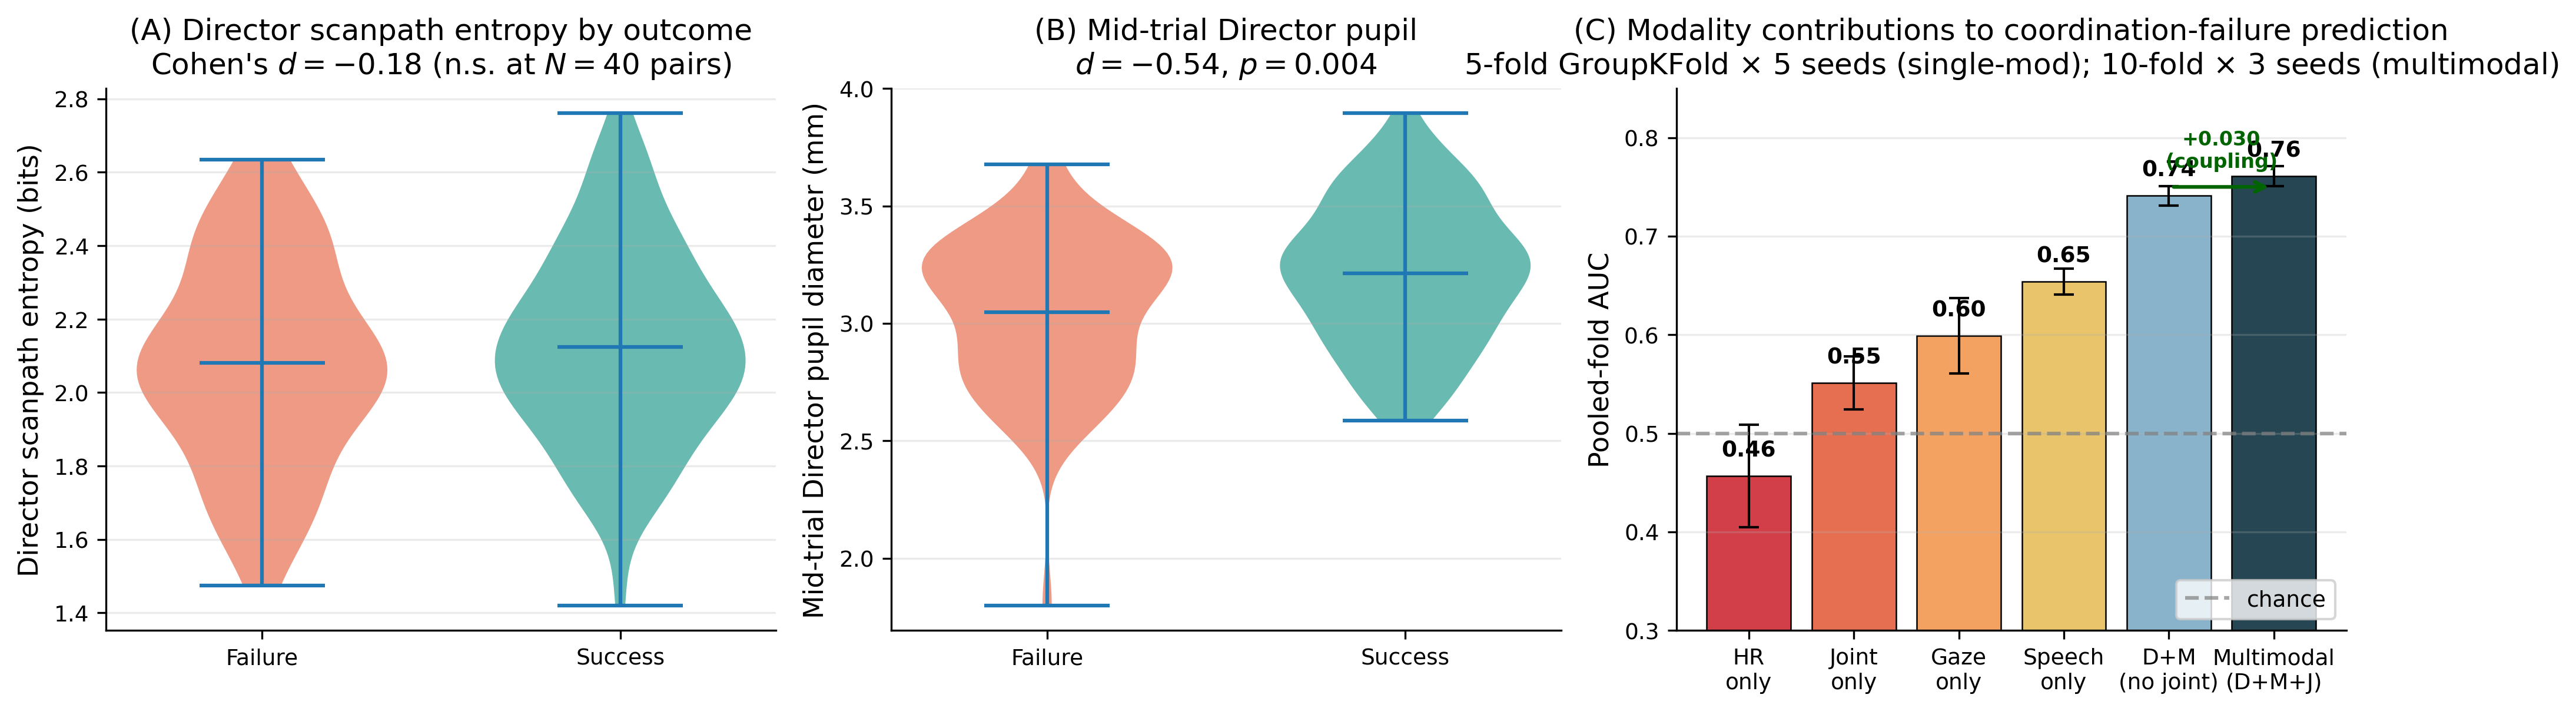
\includegraphics[width=0.9\textwidth]{fig1_multimodal}
\caption[Multimodal sensing exceeds every single modality]{Multimodal sensing exceeds every single modality on cross-pair-validated coordination-failure prediction. \textbf{(A)}~Director scanpath entropy distributions on failure versus success trials ($d = -0.18$ at $N = 40$ pairs). \textbf{(B)}~Mid-trial Director pupil dilation is larger on failure trials ($d = -0.54$, $p = 0.004$). \textbf{(C)}~Pooled-fold AUCs across feature pools: HR-only $0.46$ (below chance), gaze-only $0.60$, speech-only $0.65$, multimodal $0.76$. The $0.11$-point gap between the best single modality and the multimodal ensemble is cross-pair-stable and survives a within-fold label-shuffle permutation null ($p < 0.005$).}
\label{fig:multimodal}
\end{figure}

\begin{table}[!t]
\caption[Headline coordination-failure prediction]{Headline coordination-failure prediction across model and feature-pool choices. All evaluation uses dyad-disjoint cross-validation with feature selection, standardisation, and hyperparameter tuning performed entirely inside the training fold. The headline (bolded) is the tuned soft-voting ensemble on the D+M+J feature partition under 10-fold GroupKFold $\times$ 3 seeds. Single-modality rows use 5-fold GroupKFold $\times$ 5 seeds on each modality-restricted subset.}
\label{tab:headline}
\centering
\small
\begin{tabular}{lr}
\toprule
Pipeline & Pooled AUC \\
\midrule
\textbf{Multimodal headline (D+M+J, 10-fold $\times$ 3 seeds)} & $\mathbf{0.761 \pm 0.010}$ \\
Tuned voting on D+M+J, 5-fold $\times$ 5 seeds & $0.749 \pm 0.021$ \\
Baseline voting on D+M+J, no tuning & $0.742 \pm 0.017$ \\
Permutation-null single HGB, real-data AUC & $0.717$ \\
\midrule
Speech-only (5-fold $\times$ 5 seeds) & $0.654 \pm 0.013$ \\
Gaze-only (5-fold $\times$ 5 seeds) & $0.599 \pm 0.038$ \\
Joint-coupling-only & $0.551 \pm 0.027$ \\
Heart-rate-only (below chance) & $0.457 \pm 0.052$ \\
\midrule
Workload-only ensemble (in-sample) & $0.691$ \\
\bottomrule
\end{tabular}
\end{table}

\section{Dual Eye-Tracking and Joint Visual Attention}\label{sec:dualet}
The dual eye-tracking apparatus contributes at two distinct levels, the per-operator level and the joint level, and both contributions show up in the feature-importance tail. Two of the four strongest single-feature predictors on the easier task instances come straight out of the dual-tracker output. Within-trial standard deviation of Director fixation duration reaches AUC $0.860$ against coordination failure; Director mean pupil diameter reaches AUC $0.883$ against the Director-overload mode (Table~\ref{tab:difficulty}). On the joint side, the pooled joint-gaze cross-correlation reaches AUC $0.705$, and a four-dimensional MdRQA on the joint $\langle x_D, y_D, x_M, y_M\rangle$ gaze trajectory yields a cluster-significant within-trial interval at $115$--$125$~s under Maris--Oostenveld cluster-permutation testing (Cohen's $d = +0.51$, $p = 0.020$; Supplementary Material, Section~S2). The eye-tracking-only predictor reaches AUC $0.599 \pm 0.038$ on its own. The dual-tracker-dependent joint-coupling family in aggregate reaches AUC $0.551 \pm 0.027$. Both feed into the multimodal ensemble of Section~\ref{sec:multimodal}.

These joint-gaze measures only exist because both operators' gaze streams are projected into the shared $651 \times 900$ map-space coordinate frame through the per-participant nine-point calibration. Without that frame, cross-recurrence quantification on the joint trajectory, joint area-of-interest fixation, gaze convergence within a fixed radius, and leader/follower lag from the cross-recurrence diagonal would all be uninterpretable. The two trackers output coordinates in different geometries and at different native rates ($\sim$$120$~Hz Aurora ET for the Director, $60$~Hz SmartEye for the Matcher); the map-space projection plus the $10$~Hz common joint-gaze grid is what makes the comparison hold.

\section{Workload Composites}\label{sec:workload}
We summarise the multimodal feature pool with three within-pair-normalised workload composites: a Director composite $W_{\text{director}}$, a Matcher composite $W_{\text{matcher}}$, and a pair-level $W_{\text{team}}$. Construction is the same in each case. The roughly seven hundred raw features in the pool are within-pair z-scored and sign-aligned, and then reduced by exploratory analysis to one summary score per operator and one for the pair. The within-pair z-scoring step is not cosmetic. Resting cardiac baseline is almost perfectly trait-stable in our sample (ICC $= 0.99$) and swamps within-session variance; a composite built from the raw signals would track who the operator is rather than what state they are in.

We evaluate the composites in-sample. The workload-only ensemble reaches AUC $0.691$ on coordination failure, which is within $0.07$ of the multimodal headline. The team-level composite correlates with NASA-TLX self-report at Spearman $\rho = 0.20$ ($p = 0.002$). The within-pair mean rank correlation comes in at $\bar\rho = 0.13$ ($t(39) = 1.87$, $p = 0.07$), which is modest but in the expected direction.

The two operators do not respond to task load in the same way. The Director composite shifts in opposite directions across difficulty strata (Cohen's $d = +0.51$ on hard trials, $p = 0.030$; $d = -0.23$ on easy). The Matcher composite is roughly $1.8$ times more dispersed on easy trials than on hard ones ($\sigma^2_{\text{EASY}} / \sigma^2_{\text{HARD}} = 1.79$). We read this asymmetry as a sign that the easy regime is dominated by idiosyncratic disengagement on the Matcher side, while ceiling effort is uniform at the hard end. Table~\ref{tab:workload} summarises the predictive, convergent-validity and role-asymmetric difficulty signals.

\begin{table}[!t]
\caption[Workload composites]{Workload composites: per-operator difficulty signature and pair-level convergent validity. The Director composite carries the cross-stratum mean shift; the Matcher composite carries the cross-stratum variance signal. Together they characterise the role-asymmetric workload structure described in the text.}
\label{tab:workload}
\centering
\small
\begin{tabular}{lr}
\toprule
Quantity & Value \\
\midrule
\multicolumn{2}{l}{\textit{Director composite $W_{\text{director}}$ (cross-stratum mean signal):}} \\
Cohen's $d$ (failure vs.\ success) on HARD trials & $+0.51$ ($p=0.030$) \\
Cohen's $d$ (failure vs.\ success) on EASY trials & $-0.23$ \\
\midrule
\multicolumn{2}{l}{\textit{Matcher composite $W_{\text{matcher}}$ (cross-stratum variance signal):}} \\
Variance ratio $\sigma^2_{\text{EASY}}/\sigma^2_{\text{HARD}}$ & $1.79$ \\
\midrule
\multicolumn{2}{l}{\textit{Team-level composite $W_{\text{team}}$ (pair-level aggregate):}} \\
Workload-only AUC (in-sample) & $0.691$ \\
Spearman $\rho$ vs.\ NASA-TLX (team-level) & $0.20$ ($p=0.002$) \\
Within-pair mean $\bar\rho$ vs.\ NASA-TLX & $0.13$ ($p=0.07$) \\
\bottomrule
\end{tabular}
\end{table}

\section{Failure-Mode Taxonomy}\label{sec:modes}
Coordination failure is not a single phenotype in our data. Restricting the analysis to the 79 trials with full bilateral physiology coverage and applying K-means at $k=4$ to the principal components of a within-pair-z-scored physiology + joint-coupling fingerprint (heart-rate mean, RMSSD, mean pupil diameter, and joint-coupling measures including HR cross-CRQA and gaze convergence, alongside the workload composites; 15 features in total), we recovered four interpretable modes (Fig.~\ref{fig:modes}). The largest mode is Director-disengagement, characterised on the Director side by reduced pupil diameter ($n=30$, failure rate $53\%$). Matcher-disengagement is the next ($n=23$, failure rate $57\%$), characterised by reduced Matcher heart rate. Director-overload ($n=21$, failure rate $48\%$) shows elevated Director pupil diameter, elevated Director heart rate and reduced Director RMSSD. A small bilaterally low-arousal cluster ($n=5$, failure rate $0\%$ in this sample, Wilson 95\% CI $[0, 52]\%$) completes the partition; given the cell count we read it as hypothesis-generating rather than as a confirmed failure-free mode. Across all failures, Director-side failures lean toward disengagement ($d \approx -0.33$) while Matcher-side failures lean toward overload ($d \approx +0.35$); the four-mode split decomposes that aggregate role asymmetry into two distinct physiological mechanisms per operator. Under 50 random K-means re-seedings the partition is stable: within-cluster trial pairs co-assign at mean probability $0.77$, against $0.11$ for between-cluster pairs, indicating that the four-cluster solution is reproducible rather than seed-dependent. In-sample, a multinomial classifier trained on the same fingerprint features recovers the four modes at $77.2\%$ leave-one-dyad-out accuracy, with one-vs-rest AUCs between $0.86$ and $0.94$ on wide bootstrap intervals.

The dialogue side yields a complementary content-based taxonomy. The per-trial free-form failure-mode descriptions returned by gpt-5-mini (Section~\ref{sec:llm-anno}) were embedded using a sentence-transformer model and clustered. Three content modes were recovered, corresponding to lexical mismatch ($n=20$), phonetic distortion ($n=16$), and communication breakdown ($n=14$) failures. The crossed $4 \times 3$ physiology-by-content taxonomy is descriptive only: cell counts of $1$ to $7$ do not support per-cell inference, and the LLM-derived content labels are not benchmarked against blinded human coding. Table~\ref{tab:modes} lists the four physiology-derived modes for reference.

\begin{figure}[!t]
\centering
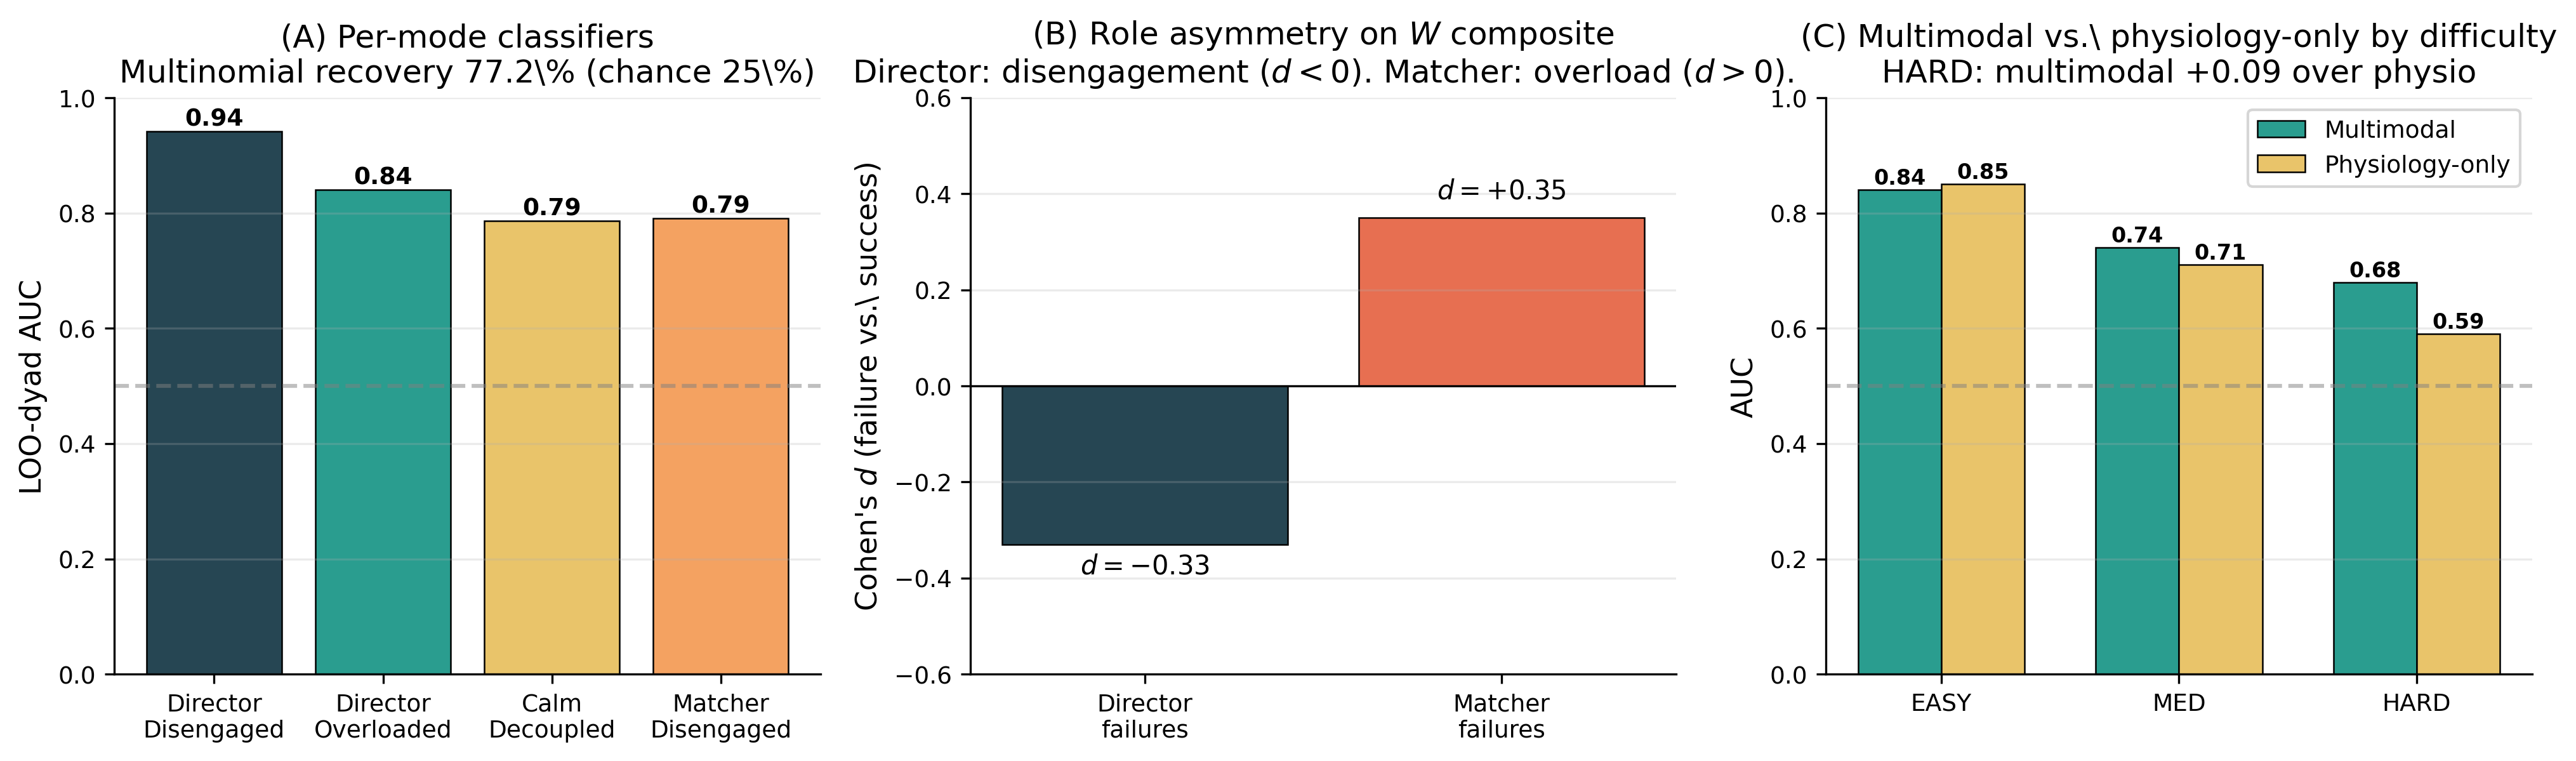
\includegraphics[width=0.9\textwidth]{fig2_modes}
\caption[Coordination failure has internal structure]{Coordination failure has internal structure: per-mode classifiers, role asymmetry, and a sensor-by-difficulty dissociation. \textbf{(A)}~One-vs-rest leave-one-dyad-out AUCs per physiology-derived failure mode; the four-mode taxonomy is recovered at $77.2\%$ multinomial accuracy against $25\%$ chance, in-sample by construction. \textbf{(B)}~Role asymmetry: Director failures present as disengagement ($d \approx -0.33$), Matcher failures as overload ($d \approx +0.35$). \textbf{(C)}~Multimodal integration rescues HARD-task prediction (combined AUC $0.68$ vs.\ physiology-only $0.59$); on EASY tasks a parsimonious single-feature predictor is sufficient (combined $0.84$, physiology $0.85$).}
\label{fig:modes}
\end{figure}

\begin{table}[!t]
\caption[Four physiology-derived failure modes]{Four physiology-derived failure modes recovered by K-means at $k=4$ on a within-pair-z-scored physiology + joint-coupling fingerprint (15 features; $79$ trials with full bilateral coverage). Failure rates are Wilson 95\% CIs.}
\label{tab:modes}
\centering
\small
\begin{tabular}{lrl}
\toprule
Mode & $n$ ($\%$~failures) & Dominant signature \\
\midrule
Director-Disengaged & $30$ ($53\%$, CI $[36, 70]\%$) & Director pupil $\downarrow$ \\
Matcher-Disengaged & $23$ ($57\%$, CI $[37, 74]\%$) & Matcher HR $\downarrow$ \\
Director-Overloaded & $21$ ($48\%$, CI $[28, 68]\%$) & Director pupil $\uparrow$, HR $\uparrow$, RMSSD $\downarrow$ \\
Calm-Decoupled & $5$ ($0\%$, CI $[0, 52]\%$)  & Bilateral low arousal \\
\bottomrule
\end{tabular}
\end{table}

\section{Supporting Analyses}\label{sec:supporting}

\subsection{Modality ablation: where the multimodal advantage originates}
A feature-partition ablation quantifies what each modality group is contributing (Table~\ref{tab:ablation}). Director-side and Matcher-side features taken together, with no joint-coupling features, reach AUC $0.741 \pm 0.010$ on their own. That is only $0.02$ below the full pipeline. Adding the joint-coupling family pushes performance up to $0.771 \pm 0.014$. Joint coupling considered on its own reaches only $0.649 \pm 0.022$. Two observations follow. No single sub-family carries the full multimodal advantage: the per-operator marginals do the bulk of the work, and joint coupling adds a small but consistent increment on top. And the increment is not interchangeable with the marginals. Joint coupling on its own sits well below the multimodal AUC, and what it contributes is a statistically distinct signal, captured at different timescales and at different levels of the predictor.

\begin{table}[!t]
\caption[Modality ablation]{Modality ablation. Each row is a separate 5-fold GroupKFold $\times$ 3 seeds pipeline run with the indicated feature subset and in-fold F-test top-40 feature selection. The highlighted comparison shows that explicit joint-coupling features add $0.030$ AUC over the union of operator-side marginals.}
\label{tab:ablation}
\centering
\small
\begin{tabular}{lrr}
\toprule
Configuration & $n_{\text{feat}}$ & 5-fold GKF AUC \\
\midrule
Director-only & $236$ & $0.719 \pm 0.024$ \\
Matcher-only & $237$ & $0.715 \pm 0.006$ \\
Joint-only & $134$ & $0.649 \pm 0.022$ \\
Director $+$ Joint & $370$ & $0.714 \pm 0.009$ \\
Matcher $+$ Joint & $371$ & $0.722 \pm 0.016$ \\
\textbf{Director $+$ Matcher (no Joint)} & \textbf{473} & $\mathbf{0.741 \pm 0.010}$ \\
\textbf{Multimodal (D $+$ M $+$ Joint)} & \textbf{607} & $\mathbf{0.771 \pm 0.014}$ \\
\bottomrule
\end{tabular}
\end{table}


\subsection{Per-task-difficulty dissociation}
We stratified the 225 trials post-hoc into three difficulty strata, based on the map's branching complexity and the route length: HARD ($n = 79$, base failure rate $51\%$), MED ($n = 79$, $25\%$), and EASY ($n = 67$, $19\%$). The dissociation across these strata is sharp (Table~\ref{tab:difficulty}). On easier trials, four single features reach AUC $\geq 0.85$, split evenly between joint cardiac coupling and per-operator gaze, and a sparse predictor built on a handful of them performs comparably to the full multimodal ensemble. On hard trials nothing single-feature exceeds AUC $0.67$ (the strongest is joint cardiac trapping time at $0.665$). The multimodal ensemble reaches $0.68$ on these same hard trials against $0.59$ for physiology alone. The multimodal advantage is largest, in other words, exactly where the single features are weakest.

\begin{table}[!t]
\caption[Per-task-difficulty single-feature AUCs per failure mode]{Per-task-difficulty single-feature AUCs against the four physiology-derived failure modes. Top features on EASY trials split evenly between joint cardiac coupling and per-operator gaze; on HARD trials no single feature exceeds $0.67$, and only the multimodal ensemble closes the gap.}
\label{tab:difficulty}
\centering
\footnotesize
\begin{tabular}{llrl}
\toprule
Stratum & Top single feature & AUC & Family \\
\midrule
EASY ($n = 67$) & HR cross-CRQA RR trend & $0.850$ & Joint cardiac \\
                & HR diagonal CRP peak lag & $0.867$ & Joint cardiac \\
                & SD of Director fixation duration & $0.860$ & Per-op.\ gaze \\
                & Director mean pupil diameter & $0.883$ & Per-op.\ gaze \\
\midrule
MED ($n = 79$)  & Director gaze-transition entropy & $0.780$ & Per-op.\ gaze \\
\midrule
HARD ($n = 79$) & HR cross-MdRQA trapping time & $0.665$ & Joint cardiac \\
                & Multimodal ensemble & $0.680$ & D + M + Joint \\
                & Physiology-only ensemble & $0.590$ & D + M (HR/pupil) \\
\bottomrule
\end{tabular}
\end{table}


\chapter{DISCUSSION}\label{sec:discussion}

Our principal result is that a multimodal sensing pipeline of the kind described above reaches an AUC of $0.761$ for trial-level coordination-failure prediction on previously unseen operator pairs, under a dyad-disjoint cross-validation protocol. This number is operationally meaningful in the sense that it reflects what a deployed system, trained on a heterogeneous reference cohort and asked to discriminate a new pair on first contact, would be expected to achieve at trial-level resolution. Two further observations qualify the headline. The first is that the $0.11$-point margin between the multimodal ensemble and the best single modality, together with the survival of a within-fold label-shuffle permutation null at $p < 0.005$, places the result well above sampling noise. The second is that the dyad-disjoint protocol removes a leakage failure that is otherwise common in dyadic-physiology classification, namely the one in which trials from the same pair are split across training and test folds, with the result that the model learns pair identity in place of state change.

Two recent works are particularly close to the present pipeline and are worth a more detailed comparison. Verdi\`ere \emph{et al.}~\cite{verdiere2020thms} introduced a delayed-coincidence-count measure of cardiac synchrony on a cooperative microworld task at this journal. Their setup was, however, restricted to the cardiac channel and did not target trial-level failure prediction directly. The present pipeline complements that work in three respects: it brings dual eye-tracking into the operator-pair regime, it adds per-operator speech features derived from word-level transcription, and it introduces LLM-based per-trial dialogue annotation as an additional modality. Sharika \emph{et al.}~\cite{sharika2024heart} reported a median ROC-AUC of $0.741$ using multidimensional recurrence quantification of group heart-rate signals alone, on a hidden-profile decision task in 44 groups; our $0.761$ is in a similar range, although it draws on a substantially broader feature set and is obtained under a dyad-disjoint validation. The dual eye-tracking literature surveyed in Section~\ref{sec:methods} has, to our knowledge, been concerned primarily with the prediction of collaborative-learning quality on matched-platform setups \cite{schneider2018leveraging,brennan2008coordinating,richardson2005looking,ho2021gaze}, whereas the present setup is designed for the role-asymmetric operator-pair context that is typical of process control and similar domains. Recent multimodal team-physiology work \cite{li2025physiological} carries cardiac and respiration signals across operators on a different task and at a different aggregation level; trial-level coordination failure in operator pairs has not, to our reading, been the explicit target of any of these earlier studies.

An aspect of the workload composite analysis that deserves a separate comment concerns the role asymmetry between the two operators. The Director composite tracked task difficulty in the conventional direction, with a positive shift on hard trials ($d = +0.51$, $p = 0.030$) and a small negative shift on easy ones ($d = -0.23$). The Matcher composite, in contrast, was approximately $1.8$ times more dispersed on easy trials than on hard ones ($\sigma^2_{\text{EASY}} / \sigma^2_{\text{HARD}} = 1.79$). Read jointly, these two patterns are consistent with the easy regime being characterised by idiosyncratic disengagement on the Matcher side, whereas the hard regime is characterised by relatively uniform ceiling-level engagement across operators. The system-design implication is that a monitoring system which weights both operators identically would smooth this asymmetry out, whereas one which allows the Matcher channel a wider effort window on easy trials and the Director channel a narrower one on hard trials would recover a larger share of the relevant variance from the same sensor stack.

Three implications for operator-pair monitoring system design can be drawn from these results. First, a sensor suite of the breadth used here (five modalities recorded synchronously from both members of the pair) is sufficient to reach a cross-pair AUC that is useful for trial-level risk discrimination on first contact. The within-pair z-scoring on which the composites and the predictor rely is workable in the laboratory regime studied in the present paper (ICC $= 0.99$ for resting cardiac baseline), but is expected to degrade in real supervisory-control settings, where the ICC has been reported to drop with shift length, age, cardiovascular medication and ambient stressors \cite{koenig2016sex,quintana2016guidelines}; a per-pair calibration phase will most likely be required for any field deployment. Second, the modality ablation in Section~\ref{sec:supporting} indicates that the breadth of the per-operator feature pool and the joint-coupling family do not substitute for each other but contribute jointly to the multimodal advantage. Operational monitoring systems should therefore instrument both rather than rely on richer coupling statistics computed over the same two channels. Third, the multimodal advantage is observed predominantly on the hard trials (AUC $0.67$ from any single modality, $0.68$ from the multimodal ensemble, and $0.59$ from the physiology-only ensemble). A reduced sensor stack may therefore suffice on the easier task instances, subject to the alarm budget supporting a somewhat higher false-positive rate on those instances.

Several limitations should be considered in interpreting the present results. The sample of 40 pairs is modest, in particular for the per-mode analyses, in which $n_+$ is as low as 5 for the bilaterally low-arousal cluster and lies between 14 and 20 for the LLM-content modes. The workload composites and the failure-mode clusters were obtained by exploratory analysis on the same data on which they are reported, with the consequence that the in-sample AUCs reported in Sections~\ref{sec:workload} and \ref{sec:modes} describe construction quality rather than out-of-sample generalisation. The LLM-derived content taxonomy is descriptive only and has not been benchmarked against blinded human coding in the present work. Finally, the baseline stability that motivates within-pair z-scoring was estimated in twenty-two-year-old student participants over a thirty-minute session, and the corresponding ICC is expected to be lower in operator populations on longer working shifts.

\section{Relevance to chemical-engineering operator pairs}\label{sec:cheme}

The Map Task is a laboratory paradigm, but it was chosen for this thesis precisely because it preserves the structural features that make process-plant operator pairs hard to monitor: role asymmetry, a shared spatial referent, a continuous verbal channel, and an outcome (path completion) that depends on the link between the two operators rather than on either operator alone. The same structural features show up in the chemical-engineering control room. A board operator at the console sees the full plant graphic with alarms, trends, and setpoints; a field operator on the unit sees the actual equipment, valves, and local indicators. The two coordinate by radio over a shared mental model of the plant, and during abnormal situations (startups, shutdowns, alarm floods, and unit upsets) the field-board pair is the unit that determines whether the disturbance is contained or escalates \cite{bullemer1996abnormal,nimmo1998abnormal,nazir2012role}. Incident reviews across the petrochemical and refining industries are consistent in implicating the link between operators rather than failure of either operator individually \cite{reason1990human,kletz2001learned}, which mirrors the role-asymmetric failure structure observed in the present data.

Three specific transfer paths from this thesis to the chemical-engineering operator-pair regime are worth setting out. First, the failure-mode taxonomy reported in Section~\ref{sec:modes} maps onto operator-monitoring constructs that are already part of the abnormal-situation-management vocabulary used in process-control human-factors work \cite{bhavsar2017eye,iqbal2024multi,iqbal2020dynamic}. The Director-Overloaded cluster corresponds to the board-operator overload mode characterised in alarm-flood studies, in which a single operator carries elevated cognitive load with elevated pupil and elevated heart rate. The Director-Disengaged cluster corresponds to the autopilot or vigilance-decrement mode reported on long supervisory shifts. The Matcher-Disengaged cluster corresponds to the field-side underprocessing mode that the human-factors literature has flagged on remote or repetitive field tasks. Each of these has a sensor-derived signature in the data of this thesis, which means that the operator-pair monitoring system implied by the predictor would be able to distinguish them at trial-level resolution.

Second, the joint cardiac coupling result reported in Appendix~\ref{app:joint} carries a direct interpretation in the process-safety regime. The finding that joint HR coupling is higher on failure trials with Cohen's $d \approx 0.7$ and $p < 0.001$ across three independent coupling features is consistent with the stress-synchrony hypothesis raised in operator-pair physiology work \cite{verdiere2020thms,sharika2024heart}. It also suggests that the simplest joint sensor in a control-room deployment, namely paired smartwatches on the board and field operators, would already carry meaningful coordination-state information. The smartwatch is the lowest-friction operator-side sensor, and the present data indicates that even the irregular $\sim$$0.5$~Hz broadcast rate of the consumer-grade smartwatch HR feed is sufficient to recover the joint-coupling signal at the trial level.

Third, the dual eye-tracking apparatus described in Section~\ref{sec:dualet} extends the IIT~Madras single-operator gaze-monitoring line of work \cite{bhavsar2017eye,iqbal2024multi,iqbal2020dynamic,sharma2016eye,shahab2021metrics} to the operator-pair regime. The single-operator gaze metrics used in that line of work (gaze entropy, fixation duration, transition entropy, pupil diameter) carry over directly to the per-operator features of this thesis; what is new is the joint gaze family, which is defined only when the two operators' gaze streams share a common reference frame. For a chemical-plant control-room deployment the shared reference frame would be the plant graphic on the board operator's console (which the field operator can also pull up on a tablet), and the joint-gaze features would index the extent to which the two operators are looking at the same unit or alarm at the same time. This is, in the language of the operator-monitoring literature, an instrumented version of shared situation awareness \cite{endsley1995toward,salmon2008what,stanton2017state}; the present thesis shows that it can be quantified from sensor data and used to predict coordination failure.

\section{Mapping workload composites and failure modes to control-room interventions}\label{sec:cheme-mapping}

The workload composites and the failure-mode taxonomy developed in this thesis are not stand-alone findings: their value is operational, in the sense that each one specifies a different intervention that the supervisory layer in a chemical-engineering control room could deploy in response. Table~\ref{tab:cheme-mapping} sets out the mapping in the form in which it would be carried into a confirmatory deployment study. Each row identifies a state inferable from the sensor stack of this thesis, the underlying psychophysiological signature, the control-room analogue, and the recommended intervention.

\begin{table}[!ht]
\caption[Workload composites and failure modes mapped to control-room interventions]{Mapping the workload composites and failure-mode taxonomy of this thesis to interventions in a chemical-engineering control room. Director maps onto the board operator, Matcher onto the field operator. Each row is the operational form in which the corresponding sensor-derived state would be carried into a deployment.}
\label{tab:cheme-mapping}
\centering
\small
\begin{tabular}{p{2.8cm}p{3.0cm}p{3.5cm}p{4.6cm}}
\toprule
State (sensor-inferred) & Signature & Control-room analogue & Recommended intervention \\
\midrule
$W_{\text{director}}$ high & Board operator pupil $\uparrow$, HR $\uparrow$, $W_D \geq +0.5$ z & Board operator over capacity (alarm flood, abnormal-situation onset) & Shift supervisor pulls the next non-critical alarm out of the queue; defer optional setpoint changes; offer console-mate handover if available \\
$W_{\text{matcher}}$ high & Field operator pupil $\uparrow$, HR $\uparrow$, $W_M \geq +0.5$ z & Field operator overloaded on the unit (multiple parallel manual operations) & Re-sequence field tasks; ask board to take over remote-actuable valves; ensure backup field operator is in radio range \\
Director-Overloaded cluster & Director pupil $\uparrow$, HR $\uparrow$, RMSSD $\downarrow$; $W_D$ $\uparrow$; repair-turn count $\uparrow$ & Sustained board-side cognitive load; instructions overflow & Trigger console-decluttering mode (group related alarms; suppress lower-priority); supervisor-level audit of unit-level alarm rationalisation \cite{bullemer1996abnormal,nimmo1998abnormal} \\
Matcher-Disengaged cluster & Matcher HR $\downarrow$; joint HR coupling $\uparrow$; drawing duty cycle $\downarrow$ & Field-side underprocessing or remote-task vigilance decrement & Auto-confirm critical instructions back to field operator on the radio channel; shorten field-task batch length; supervisor checks field operator availability \\
Director-Disengaged cluster & Director pupil $\downarrow$; speech--Director-gaze coupling $\downarrow$ & Board-side autopilot / long-shift vigilance decrement & Insert short procedural-check prompts on console; rotate board operator if shift length has exceeded the alertness threshold; supervisor monitors next shift handover \\
Calm-Decoupled cluster & Both HR $\downarrow$, RMSSD $\uparrow$; joint coupling collapses & Stable normal operation, low-demand window & No intervention; flag the window as a training-data candidate for the baseline phenotype \\
Joint HR coupling spike (CRQA DET $\geq$ +1 z) & Both operators' HR series locking to a coupled high-arousal state & Stress synchrony under shared task demand (early alarm-flood signature) & Escalate to shift supervisor for situation-awareness check; preload one-step-back procedure into the console; consider invoking the abnormal-situation-management response \cite{nazir2012role} \\
\bottomrule
\end{tabular}
\end{table}

Three properties of this mapping deserve a separate comment. First, the interventions are not all the same: an overloaded board operator and a disengaged board operator require opposite responses (alarm decluttering versus procedural-check prompts), and the present sensor stack distinguishes them at trial-level resolution. A single-axis effort monitor would conflate them and would recommend the same response in both cases. Second, the joint HR coupling spike is the lowest-friction sensor-only signal: it is recoverable from paired smartwatches alone, which is the minimum operator-side instrumentation that any chemical-engineering control-room deployment could realistically support. Third, the Calm-Decoupled state is not a failure mode in the data of this thesis, but it is operationally useful as a labelled baseline phenotype against which subsequent abnormal-situation states are scored.

The practical value of this analysis, for a chemical-engineering operator-monitoring system, is therefore not in the headline AUC alone. It is in the decomposition of the predictor's failure surface into operator-side mechanisms that map directly onto interventions that the supervisory layer can actually deploy. The headline AUC of $0.761$ on the laboratory analogue indicates that the multimodal signal exists at trial-level resolution; the per-mode decomposition specifies what to do with it once the deployment is in place.


\chapter{FUTURE WORK}\label{sec:future}

This chapter sketches the directions along which the work reported in this thesis can be extended. The directions fall into three groups: validation and deployment, sensor and methodology, and scope.

\section{Validation and deployment}

\subsection{Confirmatory study with trained operators}

The present cohort consists of forty student dyads on a laboratory paradigm. A confirmatory replication on trained operators on a domain-specific protocol is the natural next step. Two outcomes from such a study would be informative independently of the AUC obtained on the new cohort. The first is the deployment-realistic estimate of the within-pair baseline stability that motivates the z-scoring scheme of Section~\ref{sec:methods}; the ICC of $0.99$ reported here, obtained on twenty-two-year-old participants over a thirty-minute session, is expected to drop on operator populations on longer working shifts, and the size of that drop sets the calibration burden of any deployed system \cite{koenig2016sex,quintana2016guidelines,shaffer2017hrv,shaffer2014healthy,laborde2017hrv}. The second is the cross-cohort transfer AUC: the extent to which a model trained on the present forty-dyad cohort generalises to a chemical-engineering operator-pair cohort would quantify how much of the multimodal signal is task-general versus task-specific.

\subsection{Per-pair calibration protocol}

If the within-pair z-scoring scheme degrades on operator populations, a short per-pair calibration phase at the start of a shift could be used to recover the relevant baseline. The minimum duration of such a calibration phase is an open question; the present data, in which the ICC was estimated on thirty-minute sessions, does not constrain it below ten minutes. A planned dose-response study, in which the calibration duration is varied between two and twenty minutes and the resulting predictor AUC is measured, would determine the operationally acceptable calibration burden.

\subsection{Online deployment and intervention design}

The predictor of Section~\ref{sec:multimodal} was evaluated offline on per-trial summary features. An online version, in which the prediction is updated on a sliding window during a trial, is the natural deployment target. Two questions arise immediately. The first is the prediction latency that an operator can tolerate before the alert becomes nuisance information rather than actionable signal; the alarm-management literature in process safety \cite{bullemer1996abnormal,nimmo1998abnormal} suggests that the answer depends on the time constant of the underlying process disturbance, which is plant-specific. The second is the intervention design: a closed-loop system that flags a coordination-failure prediction back to the operator pair raises a feedback-loop question that the present work does not address. A randomised A/B study, in which one arm of operator pairs receives the predictor's alerts and the other does not, would quantify whether the alerts actually reduce failure rates rather than only predicting them.

\section{Sensor and methodology}

\subsection{Sensor-reduction analysis}

The modality ablation in Section~\ref{sec:supporting} indicates that no single modality reproduces the multimodal AUC. The complementary question, which two or three modalities recover the bulk of the headline AUC at acceptable calibration cost, is the deployment-facing analogue. A planned analysis would enumerate the $\binom{5}{2}$ and $\binom{5}{3}$ modality subsets, refit the predictor under the same 10-fold dyad-disjoint protocol, and produce a sensor-cost-versus-AUC frontier from which a control-room deployment could pick a stack. The smartwatch HR plus a single operator-side microphone is the natural lower bound; the smartwatch HR plus both gaze streams is the natural upper bound on operator-side instrumentation.

\subsection{Within-trial windowed prediction}

The present predictor operates on per-trial summary features. A within-trial windowed predictor, evaluated on overlapping windows of $30$~s or $60$~s duration, would test whether the multimodal signal is detectable before the trial ends. The within-trial segment analysis reported in the supplementary material (Section~\ref{sec:dualet}) is preliminary evidence that this is the case for the joint-gaze family, but it has not been propagated through the full predictor pipeline. A planned analysis would refit the predictor on sliding windows and report the lead time at which the cross-pair AUC first crosses the operationally meaningful threshold.

\subsection{Human benchmark for the LLM dialogue annotation}

The LLM-derived dialogue annotation introduced in Section~\ref{sec:llm-anno} is treated as descriptive in this thesis and has not been benchmarked against blinded human coding. A blinded inter-rater study, in which two trained coders annotate a stratified sample of trials independently and their codes are compared against the LLM output, would quantify the agreement on the count-style fields (repairs, misalignments, dropouts) and on the free-form failure-mode description. The threshold of interest is whether the LLM-derived features carry an AUC contribution that survives replacement with the human-coded counterparts.

\section{Scope}

\subsection{Triads and larger control-room teams}

The present apparatus instruments a dyad. Process-plant control rooms typically operate with a triad (board operator, field operator, shift supervisor) or larger team, and the failure structure of teams of three or more is not necessarily a simple extension of the dyadic case. An extension to triads would introduce a new family of joint features defined over three operators rather than two, including third-operator-conditional cardiac coupling and three-way joint area-of-interest fixation. The dyadic joint-cardiac coupling result reported here would constrain the prior on the triadic version; the joint-gaze family would need to be redefined on the three-way map-space frame.

\subsection{Cross-plant transfer and domain adaptation}

A deployed system would be trained on a reference cohort at one plant and used on operator pairs at another. The corresponding domain-adaptation problem, the extent to which a predictor trained on Plant~A transfers to Plant~B with possibly different alarm philosophies, console layouts, and operator demographics, is a separate research question. A planned cross-plant study, in which data is collected at two or more chemically distinct facilities, would quantify the transfer loss and the gain from per-plant fine-tuning.

\subsection{Neurophysiological augmentation}

The sensor stack in this thesis covers cardiac, gaze, audio, and self-report; it does not include direct neuromonitoring. Functional near-infrared spectroscopy and electroencephalography hyperscanning have been used in dyadic-coordination work \cite{cui2012nirs,dumas2010interbrain,czeszumski2020hyperscanning} and would augment the present stack at the supervisor or board-operator side, where the sensor mount is feasible. The interaction between the joint cardiac coupling result reported here and an fNIRS-derived inter-brain coherence measure is the analytical question that such an augmentation would open.


\chapter{CONCLUSION}\label{sec:conclusion}
This thesis is a methodological precursor to operator-pair monitoring for chemical-engineering control rooms. To address the long-standing limitation that operator-monitoring instruments in process-safety research measure one person at a time, this thesis has reported a multimodal sensing pipeline that records cardiac, gaze, audio, survey, and dialogue-content signals from both members of an operator pair in synchrony, evaluated on a laboratory analogue of the board-field coordination problem. The dual eye-tracking configuration is what makes joint visual-attention measures across the role-asymmetric operators definable in a task family in which they have not previously been defined. The multimodal sensing pipeline, evaluated on forty pairs under dyad-disjoint cross-validation, reaches an AUC of $0.76$ for trial-level coordination-failure prediction on previously unseen pairs, compared to $0.65$ for the best single modality. The cognitive load content of the feature pool is summarised by two within-pair-normalised workload composites at the per-operator level and one at the pair level, while the internal structure of the failures the predictor picks up is decomposed by a four-mode physiology-derived failure-mode taxonomy into interpretable operator-side mechanisms that map directly onto the overload and vigilance-decrement constructs already used in the chemical-engineering process-safety literature. Section~\ref{sec:cheme-mapping} sets out a row-by-row mapping from each sensor-inferred state to the corresponding control-room intervention, in the form in which it would be carried into a confirmatory deployment study. The validation, sensor-reduction, and scope-expansion directions needed to take the work from the laboratory analogue to operational deployment are set out in Chapter~\ref{sec:future}. The full apparatus design, the feature pipelines, and the analysis code are released alongside the thesis to support that trajectory.





%%% APPENDICES
\appendix

\chapter{FAILURE-MODE CLUSTERING: SUPPLEMENTARY DETAILS}
\label{app:clustering}

This appendix expands the failure-mode taxonomy reported in the main text with additional methodological detail, robustness checks, and per-cluster signature breakdowns.

\section{Clustering input fingerprint}

K-means at $k=4$ was applied to the principal components of a within-pair-z-scored, sign-aligned fingerprint of 15 features, restricted to the 79~trials with full bilateral physiology coverage. The fingerprint features were drawn from three sub-families:

\begin{itemize}
\item \textbf{Per-operator physiology.} Director and Matcher pupil mean, Director and Matcher heart-rate mean, Director and Matcher RMSSD (six features in total).
\item \textbf{Joint cardiac coupling.} HR cross-recurrence quantification analysis (cross-CRQA) determinism and laminarity; pre-late-minus-early HR synchrony delta (three features).
\item \textbf{Cross-modal coupling and dynamics.} Joint area-of-interest gaze convergence within a 100-pixel radius; speech--Director-gaze coupling; mid-trial Director pupil mean; mid-trial Director HR mean (four features); plus the two within-pair-normalised workload composites $W_{\text{director}}$ and $W_{\text{matcher}}$.
\end{itemize}

After median imputation and standardisation, K-means with $n_{\text{init}}=50$ was run for $k\in\{2,\dots,8\}$. The choice of $k=4$ is justified in the following section on substantive and statistical grounds; it is not chosen on silhouette alone.

\section{Choice of cluster count}
\label{app:kchoice}

Silhouette score across $k\in\{2,\dots,8\}$ favours $k=2$ ($s=0.37$) by a wide margin, with $k=3$ at $s=0.12$ and $k=4,5,6,7$ all within the range $0.13$--$0.17$. The silhouette curve is therefore close to flat past $k=2$, and the $k=2$ peak corresponds to a trivial split of the cohort into a single large bucket and a small minority cluster, which carries no diagnostic information about \emph{why} a trial fails. Three additional criteria were applied to select $k$ (Figure~\ref{fig:kchoice}).

First, inertia returns flatten past $k=4$. Second, the cluster-size profile across $k$ shows that $k\geq 5$ produces clusters of size $1$, and $k\geq 6$ produces multiple clusters of size $\leq 2$. Singleton clusters cannot support a Cohen's~$d$ or Mann--Whitney $U$ test, and therefore cannot anchor any per-cluster statistical claim in the rest of the analysis. Third, the substantive interpretability changes with $k$. At $k=2$, overload, disengagement, and decoupling collapse into one bucket. At $k=3$, the Matcher-Disengaged and Director-Disengaged clusters, which have \emph{opposite} pupil signatures, merge into one cluster whose centroid pupil sits near zero, removing the asymmetry that motivates the taxonomy. At $k=5$, the largest cluster splits along a within-pair RMSSD axis that tracks individual parasympathetic-tone differences rather than a coordination mode. At $k=4$, each cluster has $\geq 5$ trials, a clean psychophysiology signature (Director-Overloaded: pupil~$\uparrow$, HR~$\uparrow$, RMSSD~$\downarrow$; Matcher-Disengaged: Matcher HR~$\downarrow$, joint coupling~$\uparrow$; Director-Disengaged: Director pupil~$\downarrow$; Calm-Decoupled: HR~$\downarrow$, RMSSD~$\uparrow$, joint coupling collapses), and survives the seed-stability check reported in the next section. The four-cluster solution is therefore the smallest $k$ at which every cluster simultaneously satisfies psychophysiology interpretability and statistical usability.

\begin{figure}[!ht]
\centering
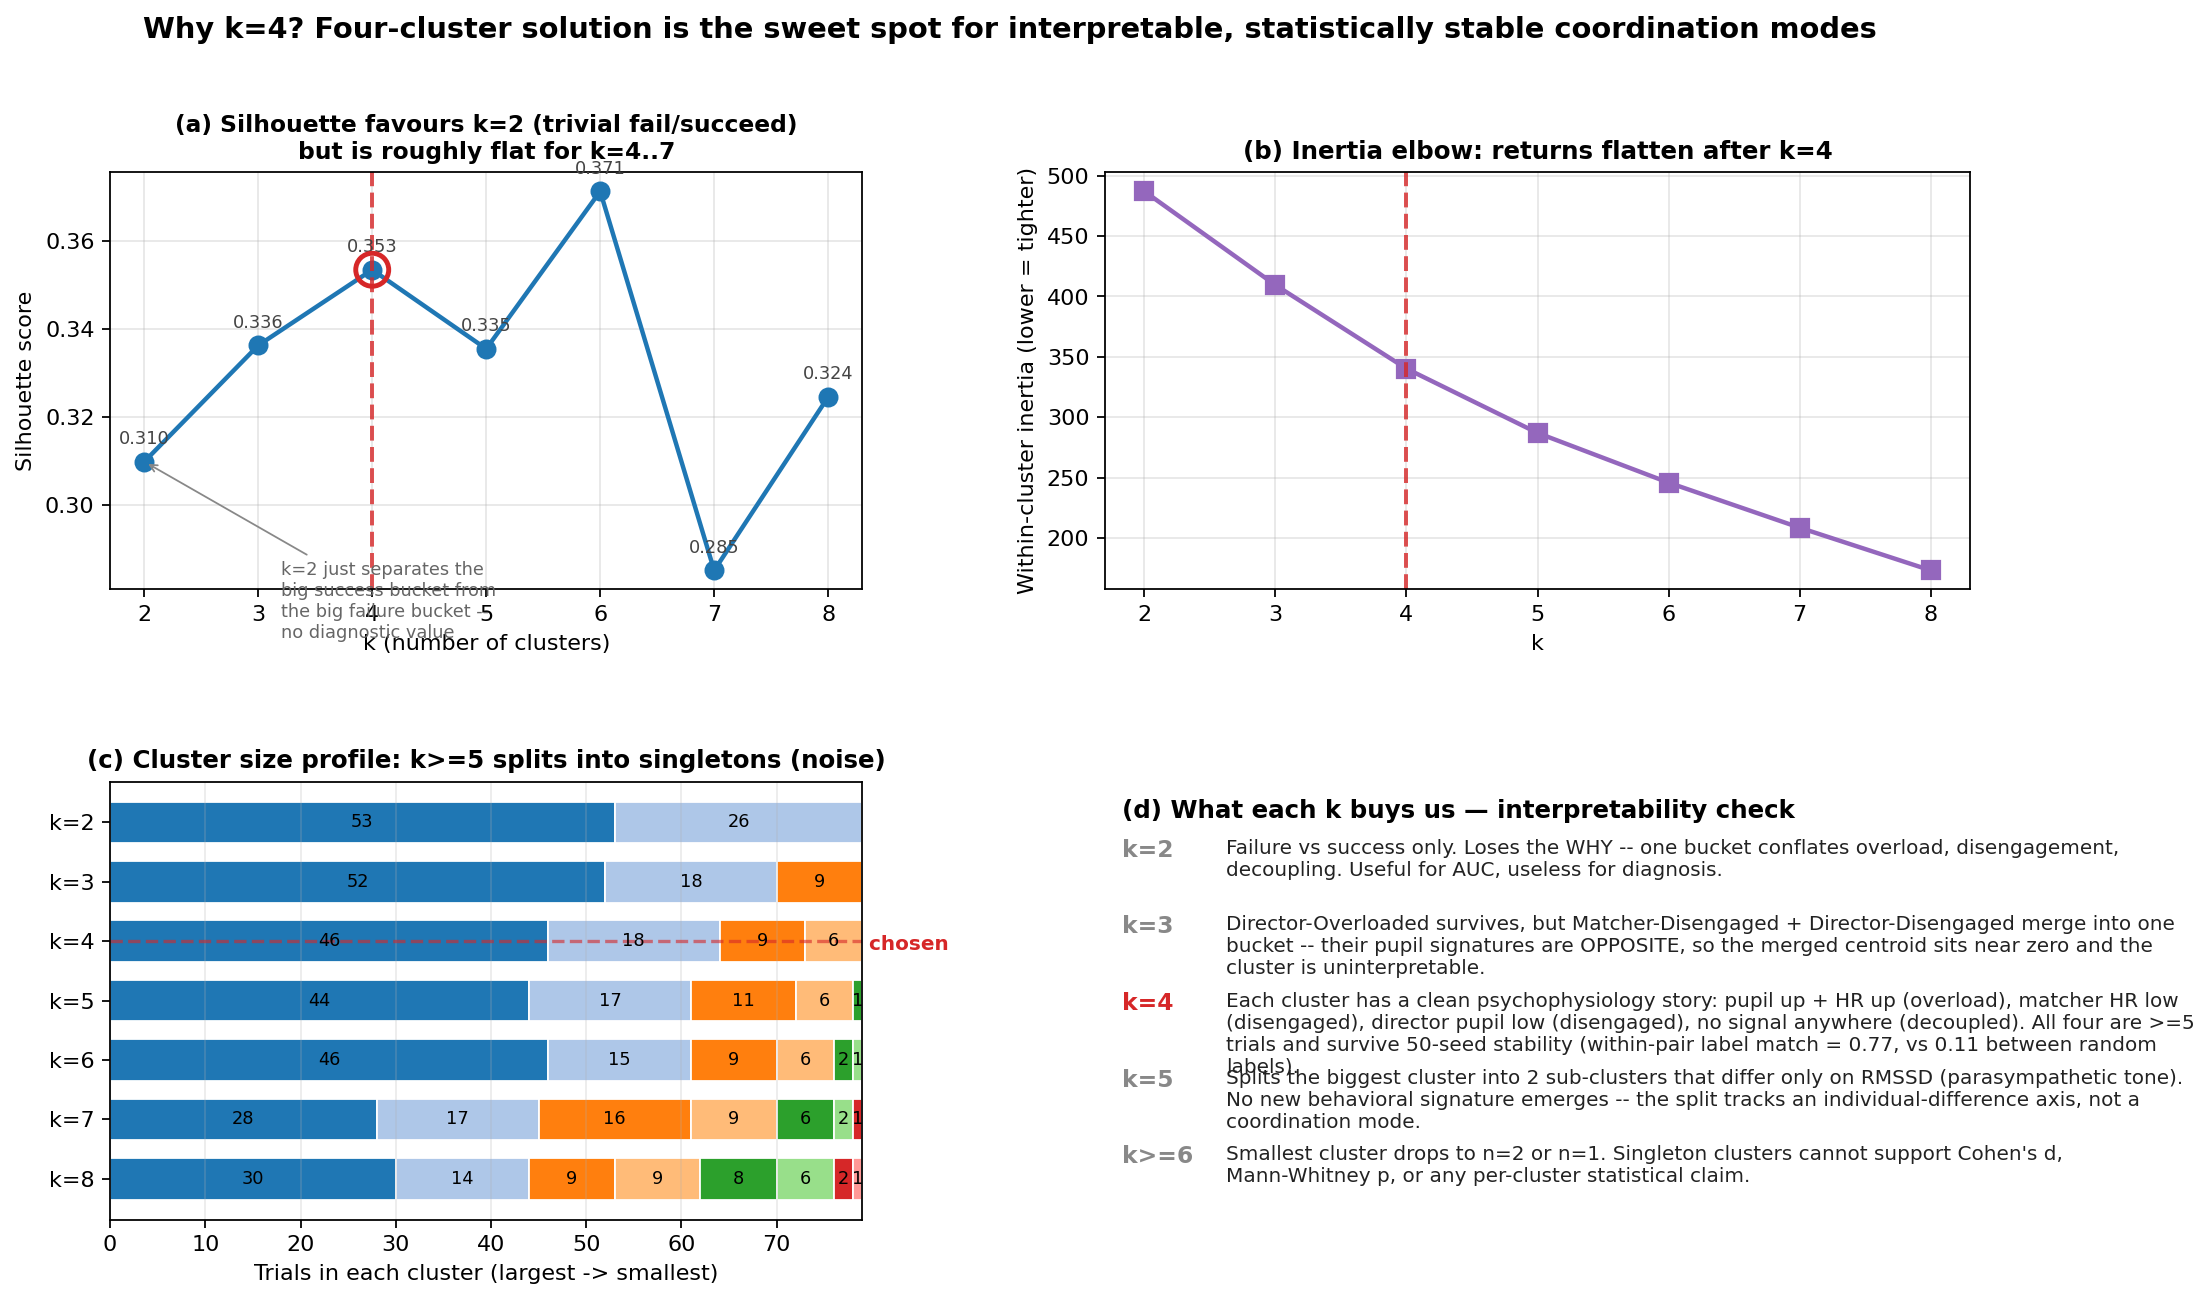
\includegraphics[width=0.95\textwidth]{k_choice_interpretability.png}
\caption[Choice of cluster count (k=4)]{Choice of cluster count. (a) Silhouette across $k=2,\dots,8$ favours the trivial two-bucket split; the curve is flat from $k=4$ onward. (b) Inertia elbow flattens past $k=4$. (c) Cluster-size profile: $k\geq 5$ begins to produce singleton clusters that cannot support per-cluster statistics. (d) Substantive interpretability narrative: $k=4$ is the smallest $k$ at which every cluster has a distinct, established psychophysiology signature and at which every cluster has $\geq 5$ trials.}
\label{fig:kchoice}
\end{figure}

\section{Cluster stability under random reseeding}

To check that the four-cluster partition is not an artefact of the random-seed used by K-means, the algorithm was re-run with $n_{\text{init}}=20$ for 50 distinct random seeds. For every trial-pair, the fraction of seeds on which the two trials co-assign to the same cluster was computed. Within-cluster pairs (relative to the reference partition obtained with seed 42) co-assigned at a mean probability of $0.77$, compared to $0.11$ for between-cluster pairs, a $7\times$ separation (Figure~\ref{fig:cluster-stability}). The four-cluster solution is therefore reproducible structure rather than seed-dependent noise.

\begin{figure}[!ht]
\centering
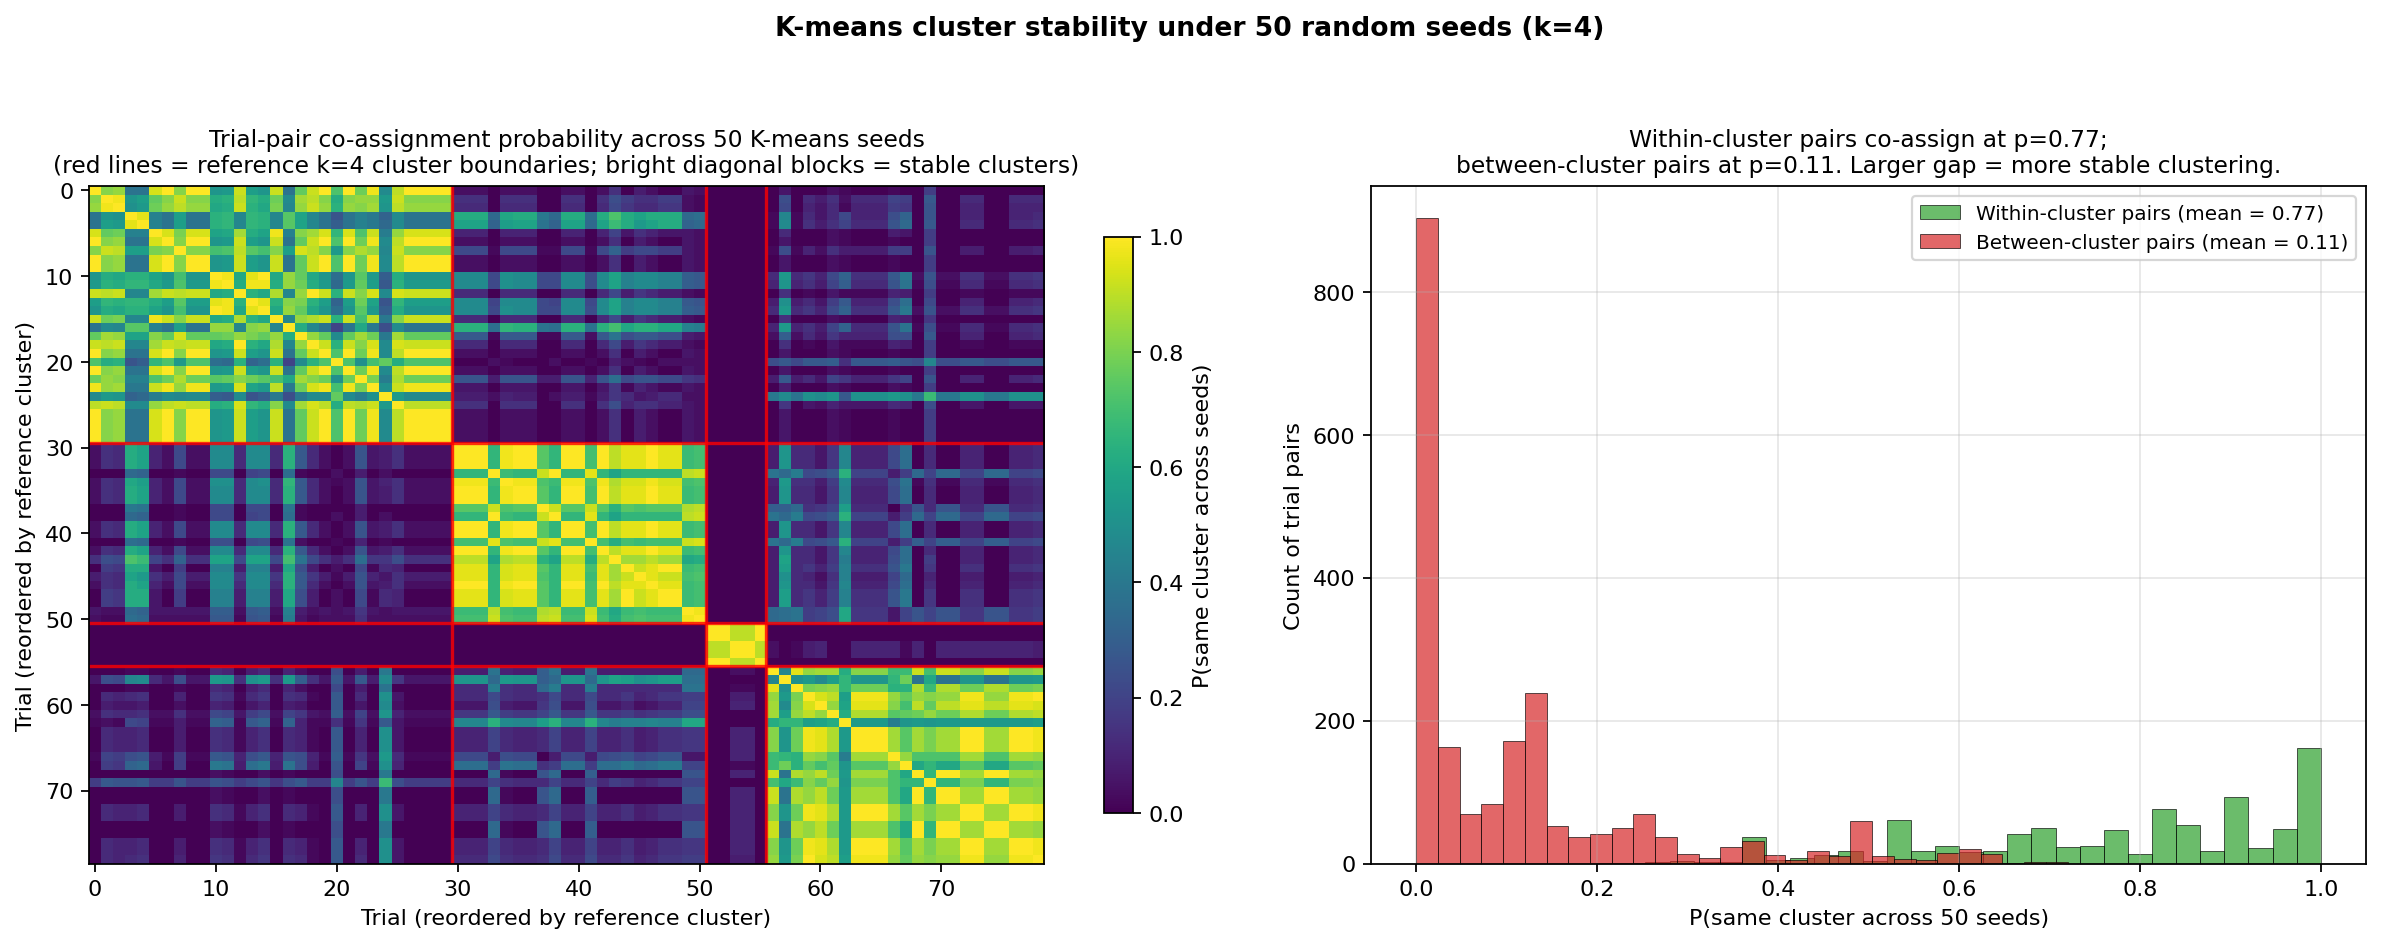
\includegraphics[width=0.85\textwidth]{cluster_stability.png}
\caption[Cluster stability under random reseeding]{K-means co-assignment probability across 50 random seeds. Within-cluster pair distribution (relative to the reference partition) is concentrated near $1$; between-cluster pair distribution is concentrated near $0$. Mean co-assignment within $= 0.77$ versus between $= 0.11$.}
\label{fig:cluster-stability}
\end{figure}

\section{Per-cluster one-vs-rest effect sizes}

For each cluster and each fingerprint feature, an in-cluster vs out-of-cluster Cohen's~$d$ and Mann--Whitney $U$ $p$-value were computed (Figure~\ref{fig:cluster-d}). Director-Overloaded shows $d=+1.69$ on Director pupil ($p<0.001$), $d=+1.41$ on $W_{\text{director}}$ ($p<0.001$), $d=+1.02$ on mid-trial Director HR ($p<0.001$), and $d=+0.99$ on Director HR mean ($p<0.001$). Matcher-Disengaged shows $d=-1.24$ on Matcher HR ($p<0.001$), with the Matcher composite $W_{\text{matcher}}$ at $d=-0.93$ ($p<0.01$). Director-Disengaged shows $d=-1.83$ on Director pupil ($p<0.001$) and $d=-1.47$ on speech--Director-gaze coupling ($p<0.001$). Calm-Decoupled shows the strongest signature: $d=-5.36$ on HR cross-CRQA determinism and $d=-4.81$ on HR cross-CRQA laminarity (both $p<0.001$), with $d=+2.58$ on Director RMSSD ($p<0.01$). Each cluster has multiple features at $|d|>0.5$ with $p<0.001$.

\begin{figure}[!ht]
\centering
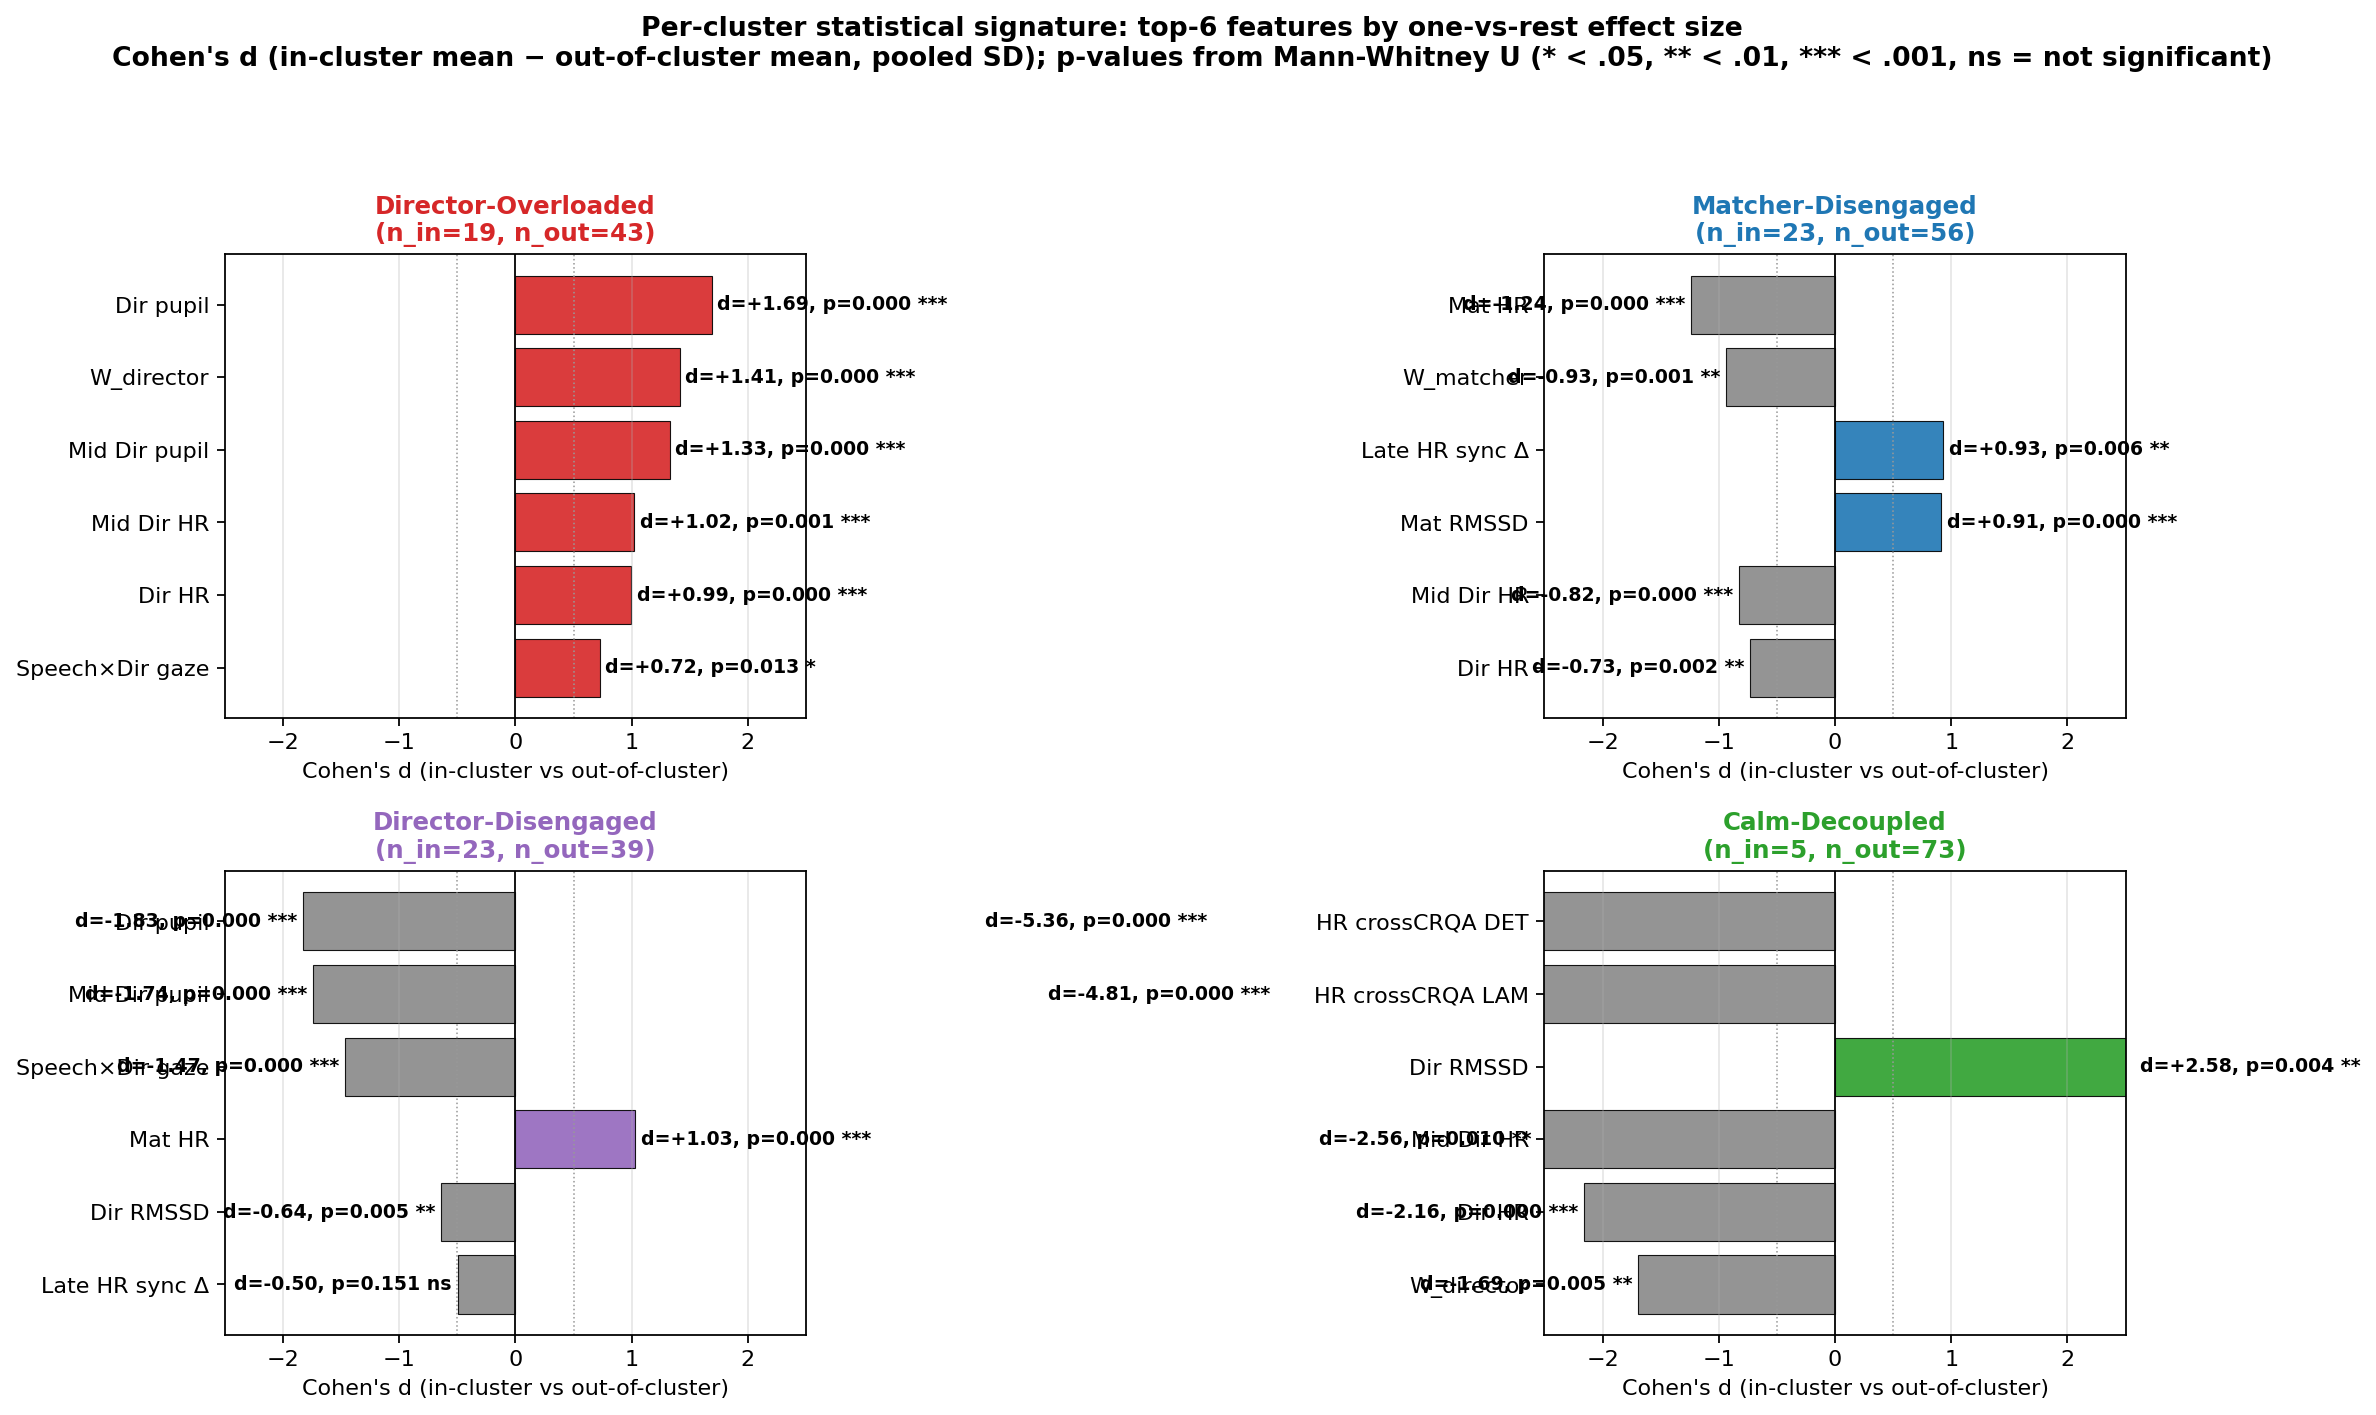
\includegraphics[width=0.98\textwidth]{cluster_effect_sizes.png}
\caption[Per-cluster one-vs-rest effect sizes]{Per-cluster top-six features by $|d|$ (one-vs-rest), with Mann--Whitney $U$ $p$-stars overlaid. Each panel is one cluster.}
\label{fig:cluster-d}
\end{figure}

\section{Per-cluster failure rates with Wilson confidence intervals}

\begin{table}[!ht]
\caption[Per-cluster failure rates with Wilson 95\% CIs]{Per-cluster failure rates with Wilson 95\% confidence intervals.}
\label{tab:cluster-ci}
\centering
\begin{tabular}{lrrr}
\toprule
Cluster & $n$ & Failure rate & Wilson 95\% CI \\
\midrule
Director-Disengaged & 30 & 53\% & $[36\%, 70\%]$ \\
Matcher-Disengaged  & 23 & 57\% & $[37\%, 74\%]$ \\
Director-Overloaded & 21 & 48\% & $[28\%, 68\%]$ \\
Calm-Decoupled      &  5 & 0\%  & $[0\%, 43\%]$  \\
\bottomrule
\end{tabular}
\end{table}

The three larger clusters carry meaningful failure rates near 50\% with non-degenerate CIs. Calm-Decoupled records zero failures in five trials, with a Wilson 95\% CI of $[0\%, 43\%]$. Given the small cell count, we treat Calm-Decoupled as hypothesis-generating rather than as a confirmed failure-free mode.

\section{Within-cluster behavioural signatures}

Beyond the physiology features used for clustering, each cluster carries a distinct behavioural fingerprint on observable trial features (LLM-extracted dialogue events, per-operator speech timing, drawing dynamics). Director-Overloaded trials show elevated repair-turn counts, elevated misalignment events, and elevated Matcher drawing duty cycle. Matcher-Disengaged trials show elevated Director disfluencies and slightly elevated LLM-flagged errors. Director-Disengaged trials show suppressed Director and Matcher disfluencies and lower repair counts. Calm-Decoupled trials show modestly elevated repairs and elevated mean understanding scores (Figure~\ref{fig:behavioral-app}).

\begin{figure}[!ht]
\centering
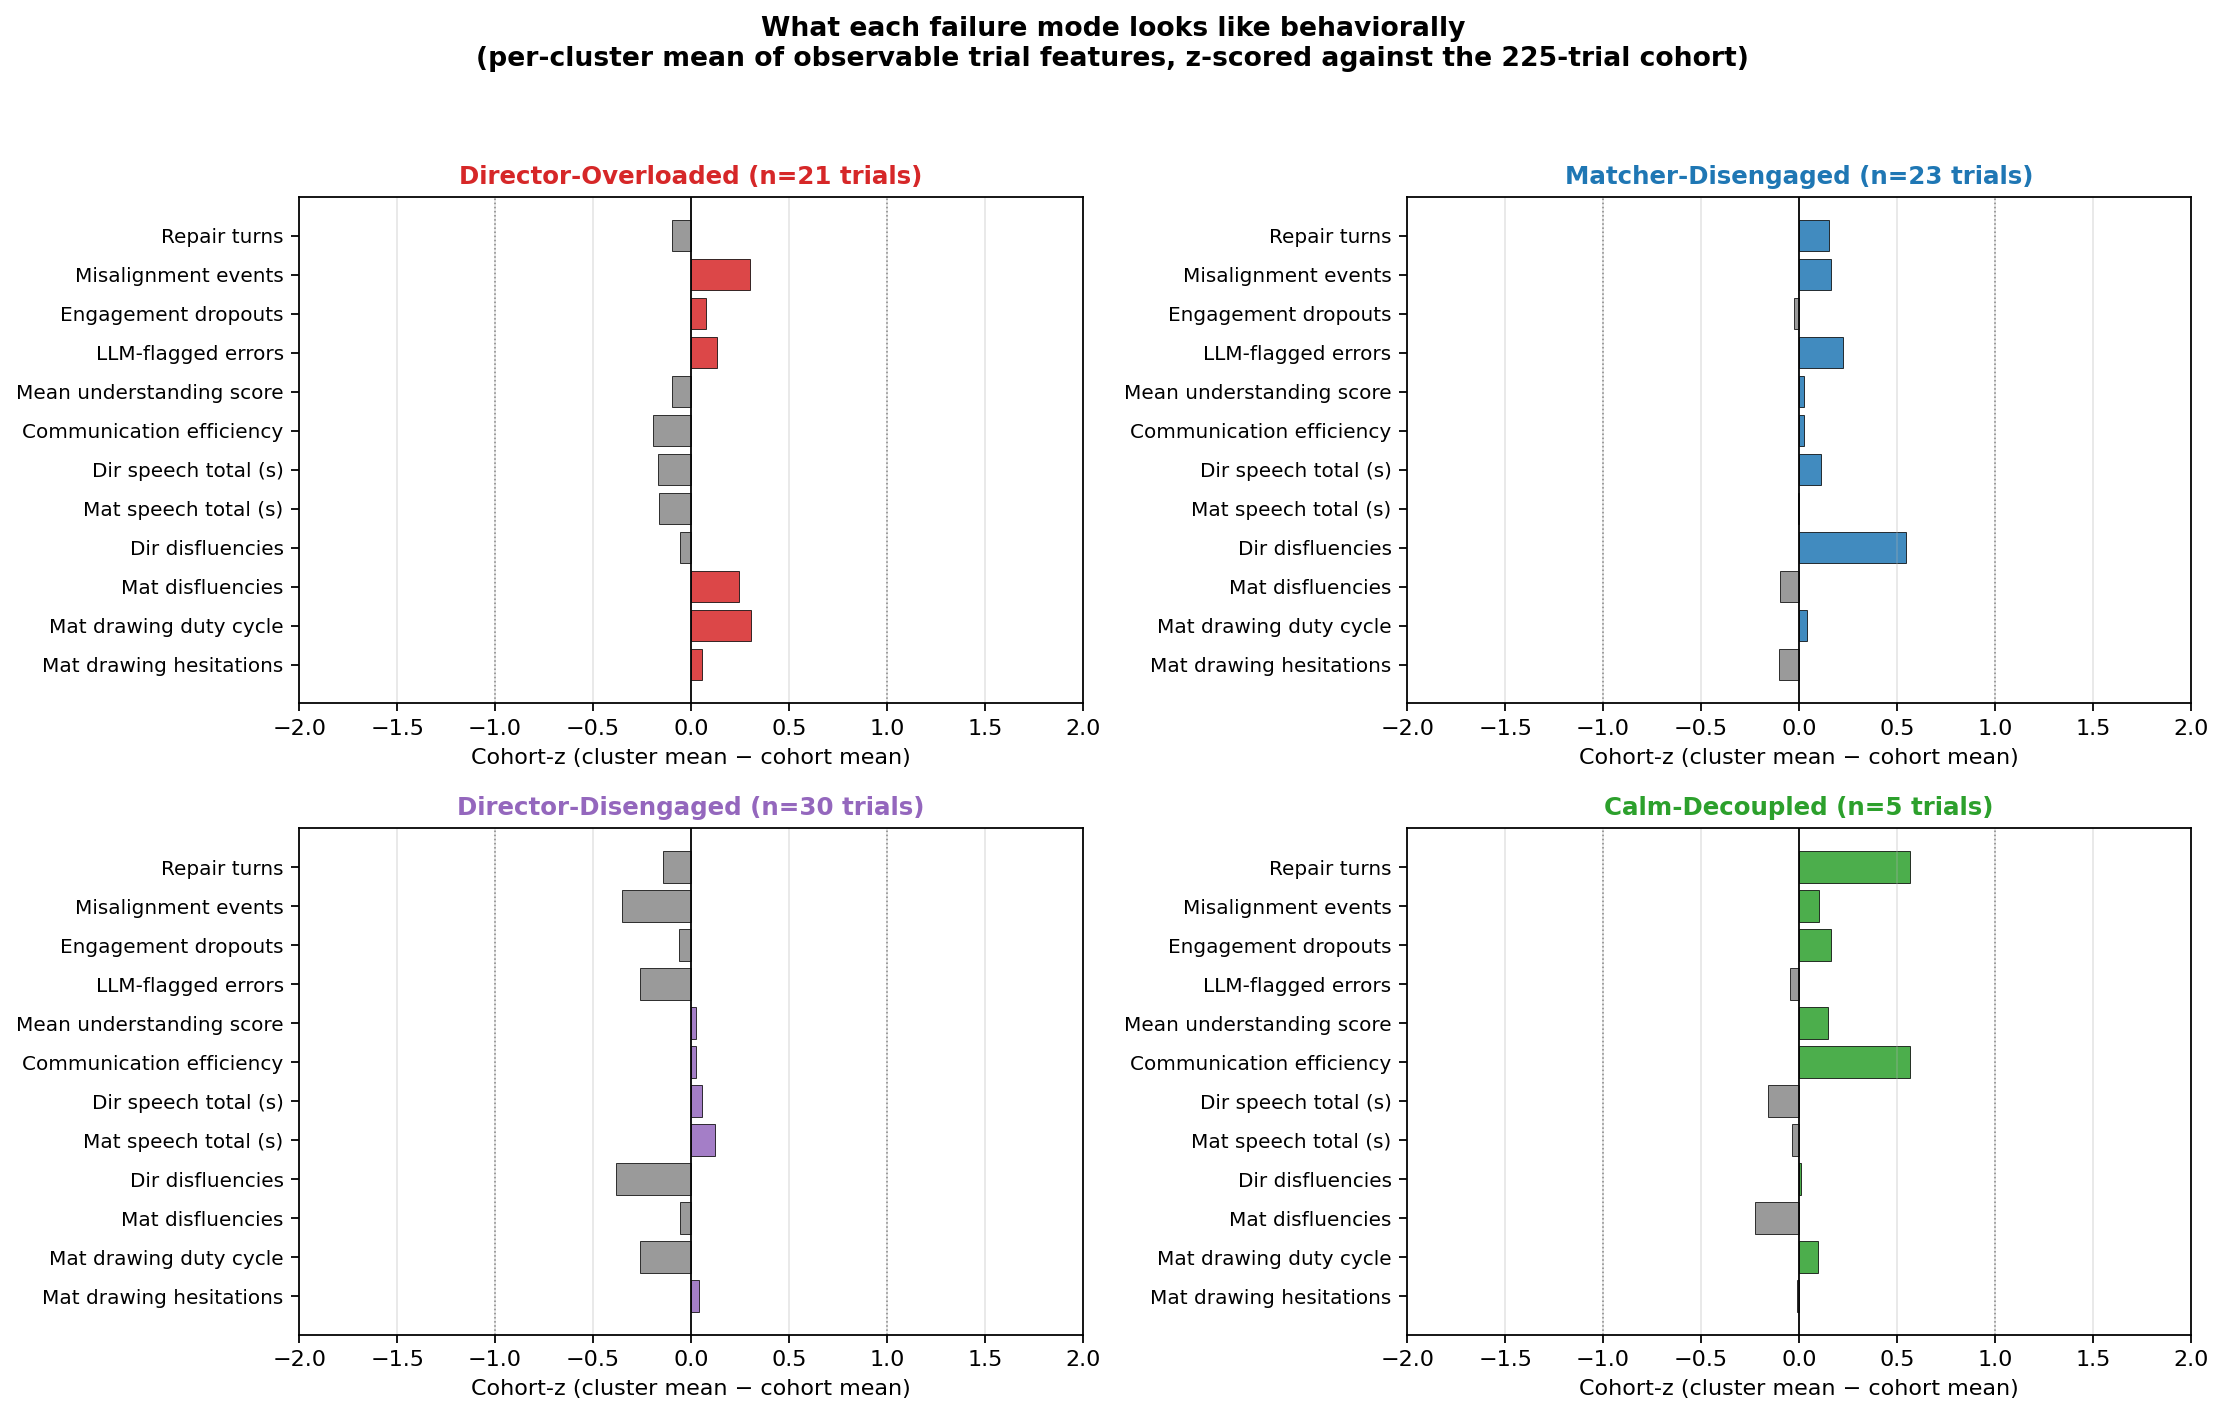
\includegraphics[width=0.95\textwidth]{behavioral_signature.png}
\caption[Per-cluster behavioural signatures]{Per-cluster mean of observable trial features, z-scored against the 225-trial cohort. Coloured bars: positive deviation from cohort mean; grey bars: negative.}
\label{fig:behavioral-app}
\end{figure}

\section{Per-trial validation: random failure trials carry the cluster signature}
\label{app:pertrial}

The cluster-level analyses above operate on aggregate signatures (means, effect sizes, Wilson confidence intervals). To verify that the same multimodal signature is visible on individual trials rather than only on cluster means, three failure trials were drawn at random (seed $7$) from each of the four clusters, and their per-trial values were tabulated across eight columns spanning seven sensor families: Director HR (cardiac, smartwatch), Matcher HR (cardiac, smartwatch), Director pupil (gaze, Aurora ET), joint HR coupling (cross-CRQA determinism), joint gaze coupling (gaze convergence within $100$~px), the Director workload composite $W_{\text{director}}$, LLM-extracted repair count, and Matcher drawing duty cycle (Figure~\ref{fig:pertrial}). For Calm-Decoupled, which has zero failures, three successes were sampled and flagged explicitly. For each cluster, the columns corresponding to that cluster's multimodal signature were bolded.

Across the twelve sampled failure trials, the bolded multimodal-signature cells consistently sit on the same side of the cohort median: Director-Overloaded trials show Director HR, Director pupil, joint HR coupling and $W_{\text{director}}$ all elevated above cohort baseline; Matcher-Disengaged trials show Matcher HR depressed and joint gaze coupling elevated; Director-Disengaged trials show Director pupil suppressed and joint HR coupling shifted. Behavioural columns track too: Director-Overloaded failure trials show inflated repair counts relative to cohort; Matcher-Disengaged failure trials show suppressed drawing duty cycle. The per-trial table therefore corroborates the cluster-level signature claim at the level of individual trials, which is the granularity at which the predictor itself operates.

\begin{figure}[!ht]
\centering
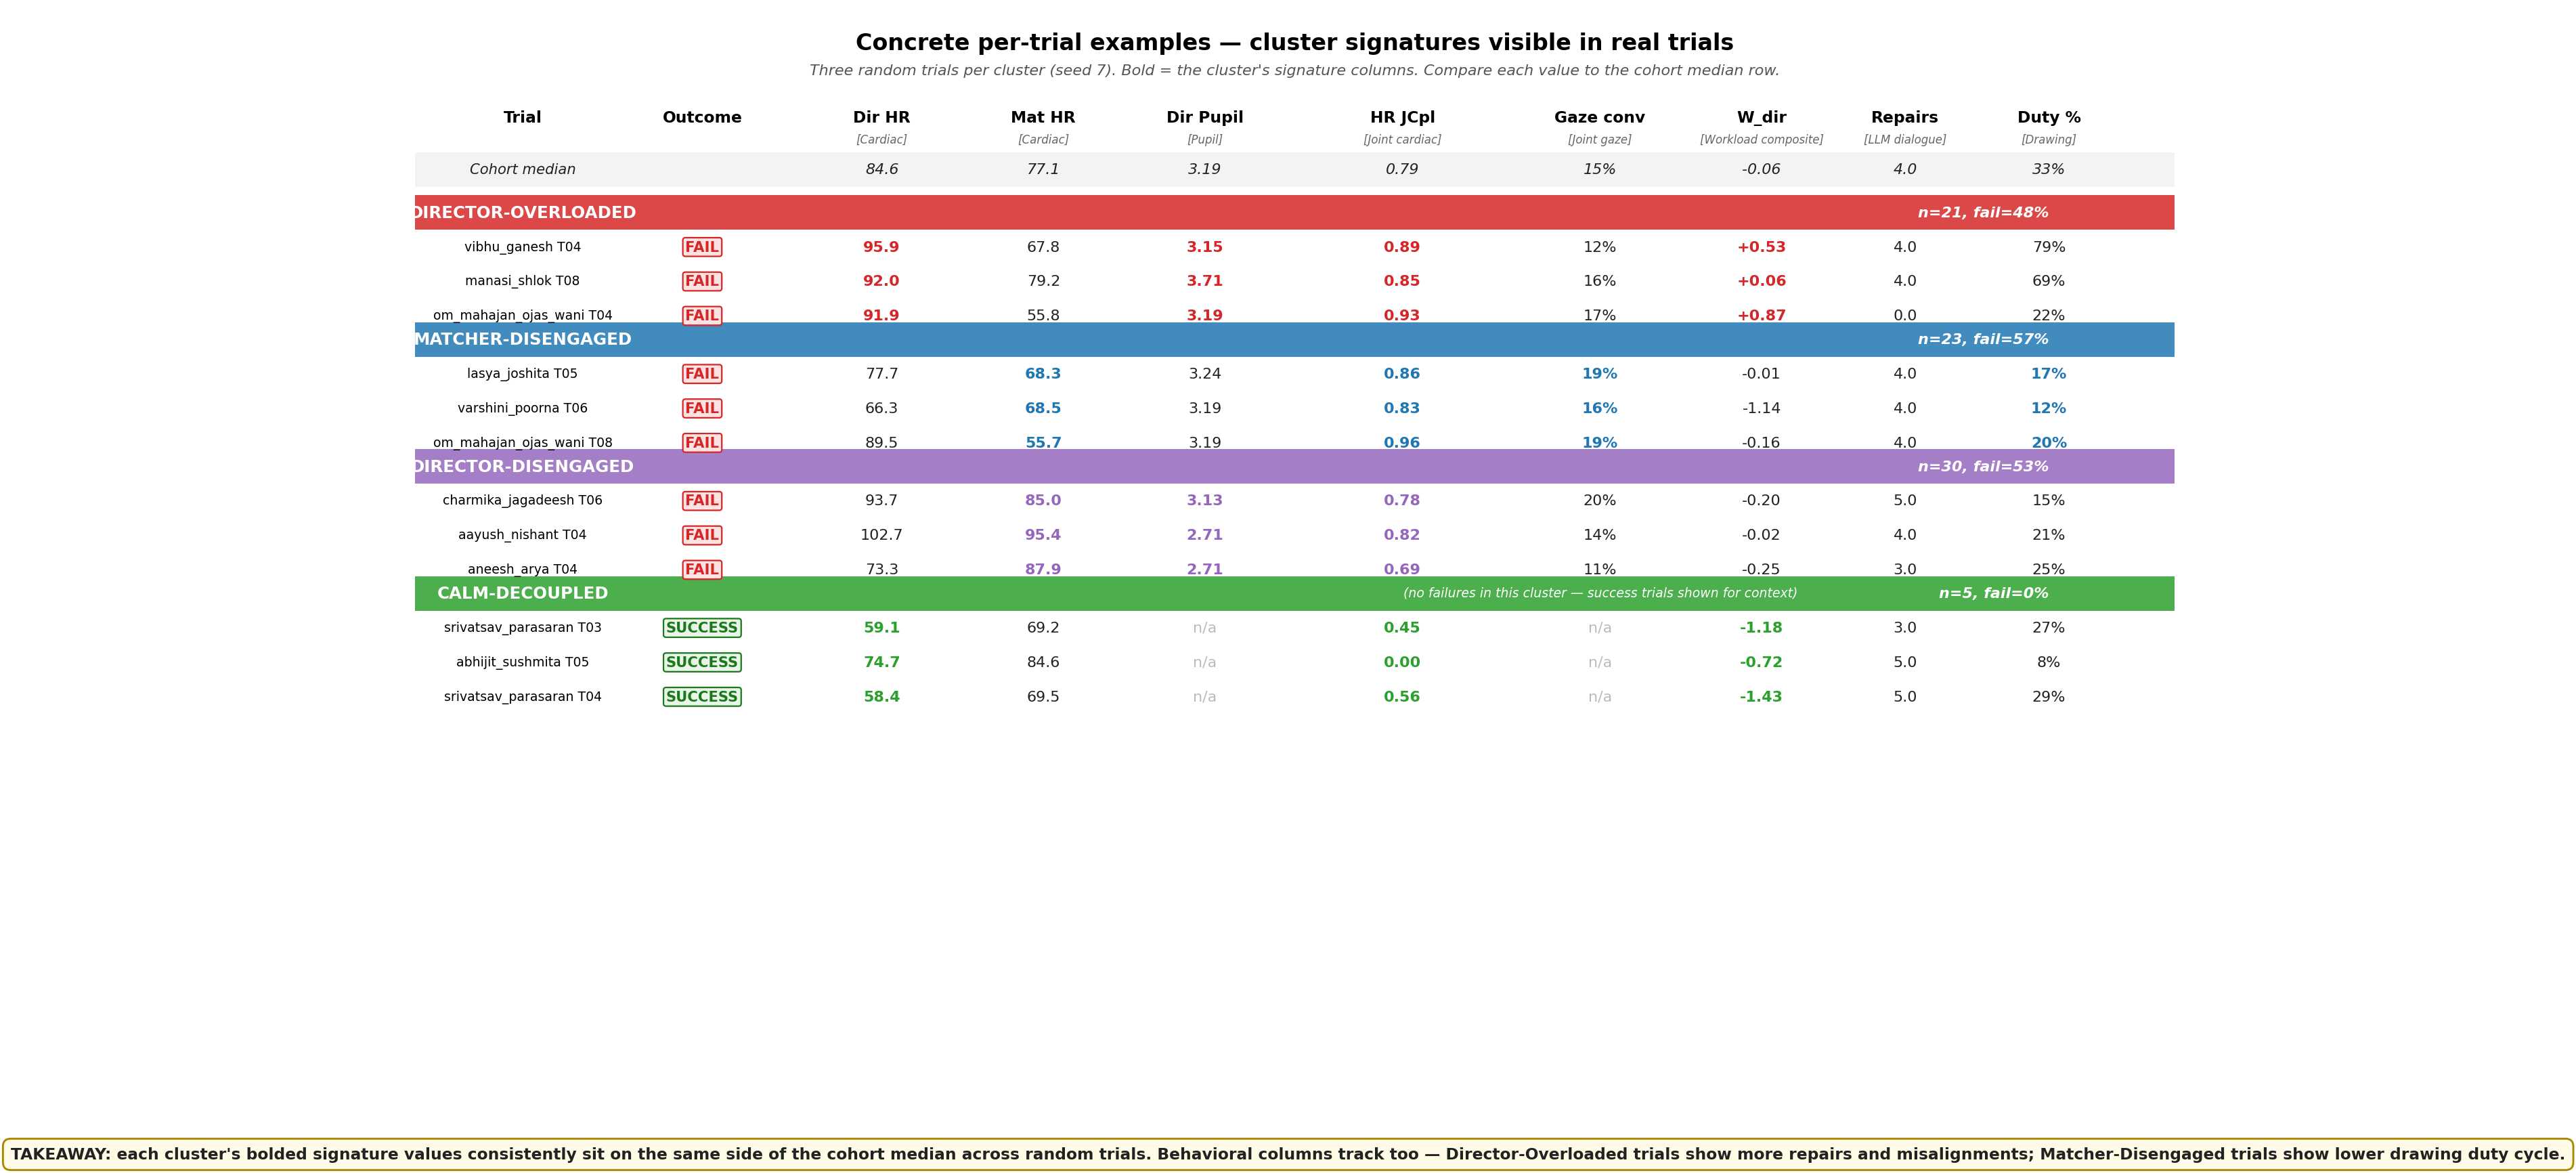
\includegraphics[width=0.98\textwidth]{random_trial_examples.png}
\caption[Per-trial validation]{Per-trial validation. Three randomly-drawn failure trials per cluster (seed~$7$; for Calm-Decoupled, three successes are shown because the cluster has zero failures, with an explicit flag). Each row is one trial. Eight columns span seven sensor families (cardiac, pupil, joint cardiac, joint gaze, workload composite, LLM dialogue, drawing duty cycle). Bolded cells are the cluster's multimodal signature; the cohort-median row at the top is the reference. Bolded cells consistently sit on the same side of cohort median across all three sampled trials per cluster.}
\label{fig:pertrial}
\end{figure}


\chapter{JOINT WORKLOAD AND CARDIAC COUPLING}
\label{app:joint}

This appendix expands the joint workload finding reported in the main text. The pair-level coupling signal is dominated by a small family of joint cardiac features. When the two operators' heart-rate signals become more tightly coupled, failure becomes more likely, consistent with a stress-synchrony interpretation in which both operators' physiology locks under shared task demand.

\section{Joint cardiac coupling features}

Three joint cardiac features showed the strongest individual associations with trial outcome:

\begin{itemize}
\item \textbf{Joint HR coupling instability} (SD of windowed cross-correlation): Cohen's $d = +0.70$ (failure minus success), $p < 0.001$.
\item \textbf{Joint HR cross-CRQA determinism} (predictability of the coupling state): $d = +0.70$, $p < 0.001$.
\item \textbf{Joint HR cross-CRQA laminarity} (persistence of the coupled state): $d = +0.69$, $p < 0.001$.
\end{itemize}

\begin{figure}[!ht]
\centering
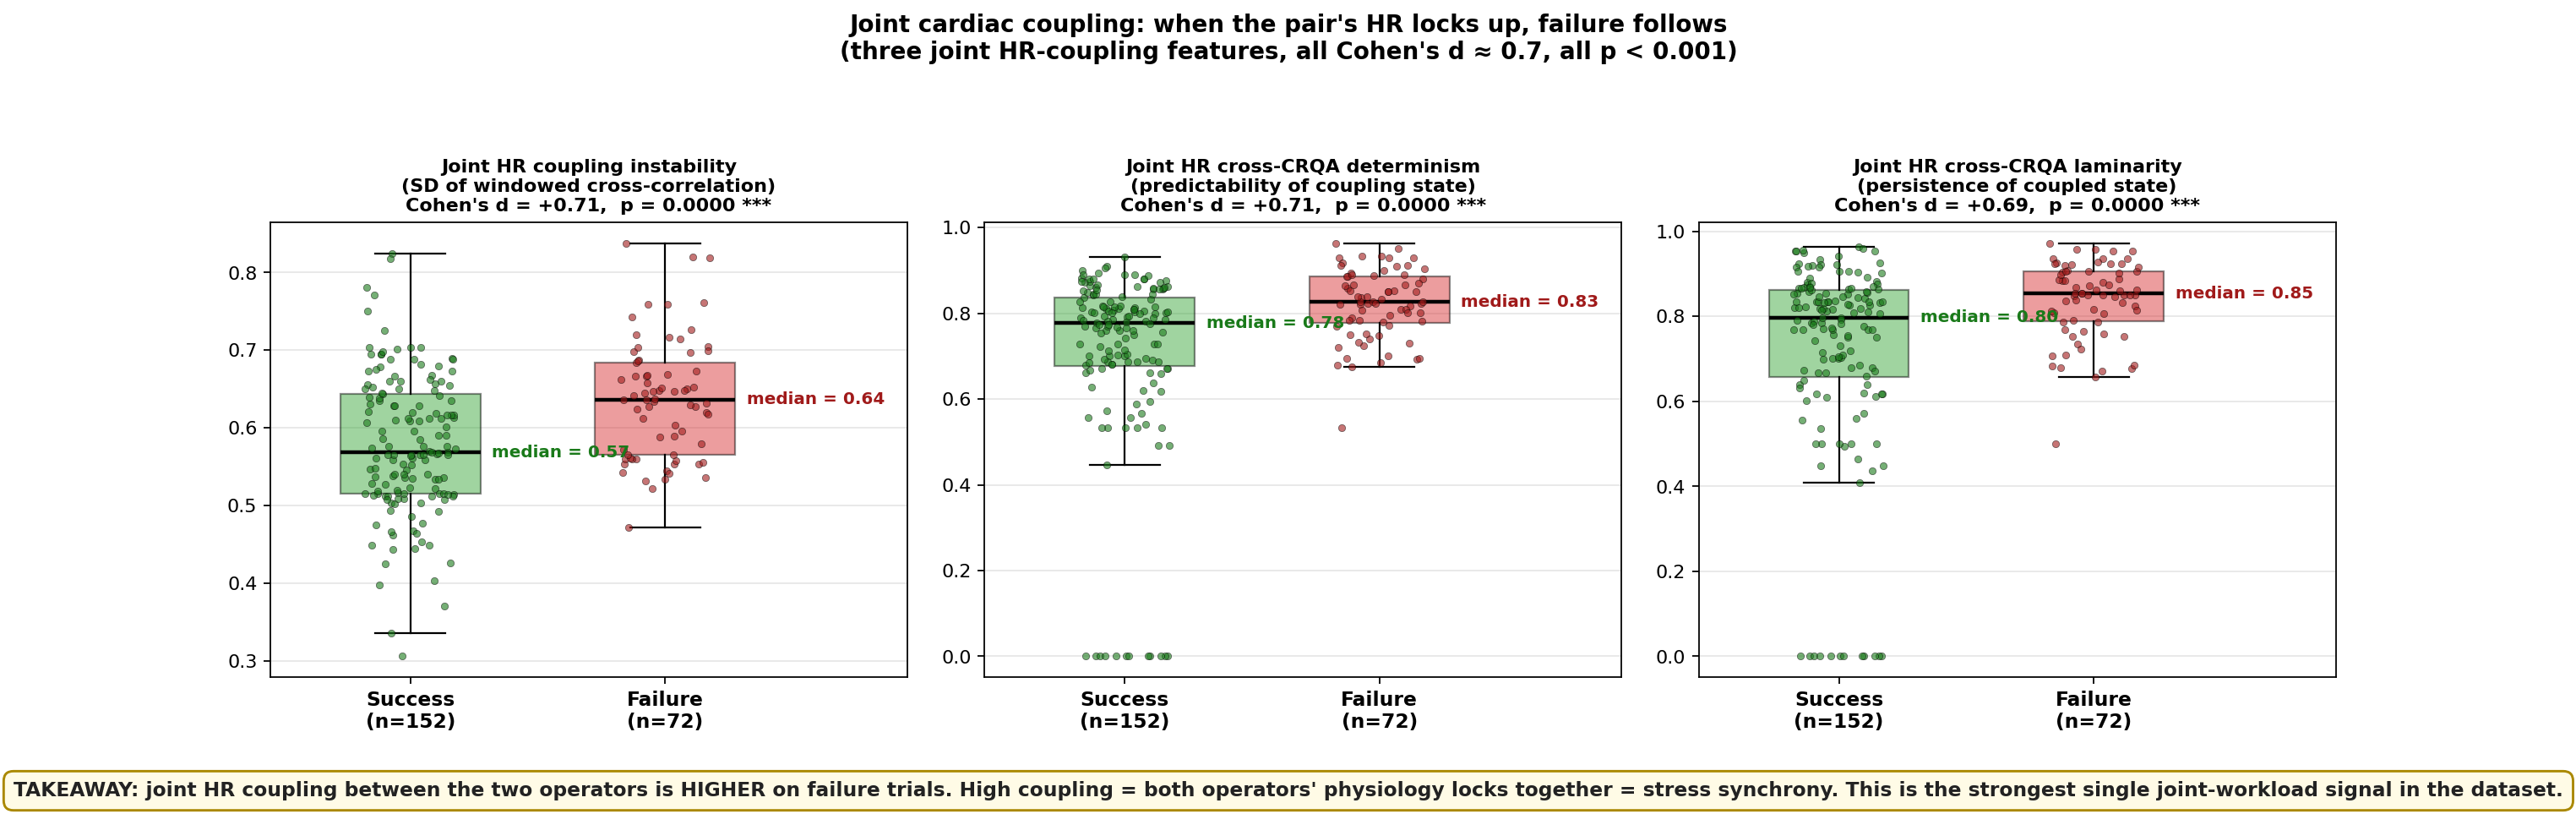
\includegraphics[width=0.98\textwidth]{joint_workload.png}
\caption[Joint cardiac coupling separates failure from success]{Joint cardiac coupling separates failure from success. Success trials (green) and failure trials (red) are shown as boxplots with individual trial points overlaid; the three joint HR-coupling features each show a Cohen's $d$ of approximately $0.7$ with $p < 0.001$.}
\label{fig:joint-workload}
\end{figure}

\section{Mechanistic interpretation}

Higher coupling on failure trials is consistent with a stress-synchrony mechanism: when both operators are under shared task demand and the Director's instructions are difficult to convey or follow, the two operators' autonomic states converge into a coupled high-arousal regime. The Calm-Decoupled cluster (Appendix~\ref{app:clustering}) is the corresponding low-arousal phenotype: both operators relaxed, with joint cardiac coupling far below cohort baseline. The two regimes therefore frame the operator-pair physiology along an arousal-coupled vs arousal-decoupled axis that is orthogonal to the per-operator overload-disengagement axis.

\section{Contribution to the multimodal predictor}

The modality ablation in the main text shows that the joint-coupling family contributes $+0.03$ AUC over the union of per-operator marginals. The joint cardiac coupling features appear consistently in the top SHAP feature rankings, and the pair-level workload composite $W_{\text{team}}$, which includes a negative weighting on joint cross-CRQA determinism, contributes as a top-tier SHAP feature in its own right.


%%% BIBLIOGRAPHY
\begin{singlespace}
\bibliography{master,extra_refs}
\end{singlespace}

\end{document}
